\section{Intégrale de Lebesgue}

The previous chapter built three objects --- a tribu, a mesure, a mesurable
function --- and stopped just short of using them. This chapter uses them: nous
allons maintenant définir une intégrale par rapport à une mesure. C'est
l'\textbf{intégrale de Lebesgue} (\textit{Lebesgue integral}), beaucoup plus générale que l'intégrale de Riemann, in two
independent directions: elle permet d'intégrer beaucoup plus de fonctions, et par
rapport à n'importe quelle mesure, pas uniquement la mesure ``uniforme'' utilisée
habituellement, qui correspond à la mesure de Lebesgue.\\

The idea is a single change of axis. Riemann cuts the \emph{domain} into small
intervals and multiplies the width of each by a value of $f$ on it. Lebesgue cuts the
\emph{range} into small intervals and multiplies the length of each level band by the
mesure of the set of points where $f$ takes a value in that band. De manière
schématique, l'intégrale de Lebesgue est définie à partir d'une discrétisation selon
l'axe des ordonnées (les différentes valeurs prises par la fonction à intégrer)
plutôt que selon l'axe des abscisses (l'ensemble de définition de la fonction): that
is the whole of the construction; everything below is bookkeeping.

\begin{figure}[h!]
  \centering
  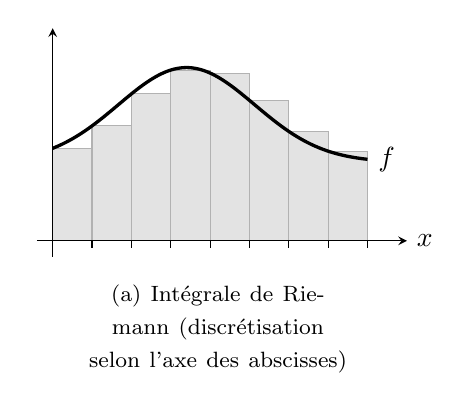
\begin{tikzpicture}[scale=1.0,>=stealth]
    % --- Riemann: vertical slabs ---
    \fill[gray!22] (0,0) rectangle (0.5,1.175);
    \fill[gray!22] (0.5,0) rectangle (1.0,1.459);
    \fill[gray!22] (1.0,0) rectangle (1.5,1.866);
    \fill[gray!22] (1.5,0) rectangle (2.0,2.168);
    \fill[gray!22] (2.0,0) rectangle (2.5,2.130);
    \fill[gray!22] (2.5,0) rectangle (3.0,1.783);
    \fill[gray!22] (3.0,0) rectangle (3.5,1.389);
    \fill[gray!22] (3.5,0) rectangle (4.0,1.138);
    \draw[gray!60] (0,0) rectangle (0.5,1.175);
    \draw[gray!60] (0.5,0) rectangle (1.0,1.459);
    \draw[gray!60] (1.0,0) rectangle (1.5,1.866);
    \draw[gray!60] (1.5,0) rectangle (2.0,2.168);
    \draw[gray!60] (2.0,0) rectangle (2.5,2.130);
    \draw[gray!60] (2.5,0) rectangle (3.0,1.783);
    \draw[gray!60] (3.0,0) rectangle (3.5,1.389);
    \draw[gray!60] (3.5,0) rectangle (4.0,1.138);
    \draw[->] (-0.2,0) -- (4.5,0) node[right] {$x$};
    \draw[->] (0,-0.2) -- (0,2.7);
    \draw[very thick,domain=0:4,samples=120,smooth]
      plot (\x,{1+1.2*exp(-(\x-1.7)*(\x-1.7)/1.5)}) node[right] {$f$};
    \foreach \t in {0,0.5,1.0,1.5,2.0,2.5,3.0,3.5,4.0}
      \draw (\t,0) -- (\t,-0.09);
    \node[text width=4.6cm,align=center] at (2.1,-1.12)
      {\footnotesize (a) Intégrale de Riemann (discrétisation selon l'axe des
       abscisses)};
  \end{tikzpicture}
  \hfill
  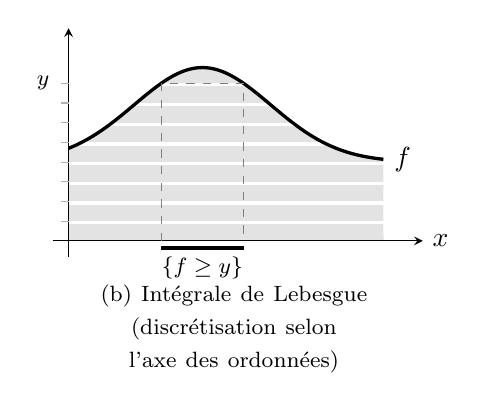
\begin{tikzpicture}[scale=1.0,>=stealth]
    % --- Lebesgue: horizontal bands ---
    \begin{scope}
      \clip (0,0) -- plot[domain=0:4,samples=120,smooth]
        (\x,{1+1.2*exp(-(\x-1.7)*(\x-1.7)/1.5)}) -- (4,0) -- cycle;
      \foreach \k in {0,1,2,3,4,5,6,7,8}
        \fill[gray!22] (0,{0.25*\k}) rectangle (4,{0.25*\k+0.21});
    \end{scope}
    \draw[->] (-0.2,0) -- (4.5,0) node[right] {$x$};
    \draw[->] (0,-0.2) -- (0,2.7);
    \draw[very thick,domain=0:4,samples=120,smooth]
      plot (\x,{1+1.2*exp(-(\x-1.7)*(\x-1.7)/1.5)}) node[right] {$f$};
    \foreach \k in {1,2,3,4,5,6,7,8}
      \draw[gray!60] (0,{0.25*\k}) -- (-0.09,{0.25*\k});
    % the level set of one band, read back on the x-axis
    \draw[very thick] (1.177,-0.09) -- (2.223,-0.09);
    \node at (1.70,-0.34) {\footnotesize $\{f \geq y\}$};
    \draw[gray,dashed] (1.177,0) -- (1.177,2.0) -- (2.223,2.0) -- (2.223,0);
    \node[left] at (-0.12,2.0) {\footnotesize $y$};
    \node[text width=4.6cm,align=center] at (2.1,-1.12)
      {\footnotesize (b) Intégrale de Lebesgue (discrétisation selon l'axe des
       ordonnées)};
  \end{tikzpicture}
  \vspace{0.5cm}
\end{figure}

\medskip
The price of the change is that the level set $\{f \geq y\}$ has to be mesurable for
its mesure to exist, which is why measurability was defined first. The reward is
that the class of integrable functions becomes stable under pointwise limits, and
that is what the three convergence theorems of this chapter say.

\subsection{Définition}

Soit $(\Omega,\mathcal{F})$ un espace mesurable.

\begin{definition}[Fonction étagée (\textit{simple function})]
  Une fonction $f$ mesurable de $(\Omega,\mathcal{F})$ vers
  $(\reals,\mathcal{B}(\reals))$ est dite \textbf{étagée} si elle prend un nombre
  fini de valeurs.
\end{definition}

Une telle fonction s'écrit :
\[
  f = \sum_{i=1}^{n} \alpha_{i} \indic_{A_{i}},
\]
où $\alpha_{1},\ldots,\alpha_{n}$ sont les valeurs distinctes et non-nulles prises
par $f$, et pour tout $i$, $A_{i} = f^{-1}(\{\alpha_{i}\})$. Notons que, la fonction
$f$ étant mesurable, each $A_{i}$ belongs to $\mathcal{F}$; this is the only place
measurability is used, and it is what makes the next definition legal. This
decomposition is called the canonical form, and it will be referred to below simply
as writing $f$ in the form above.

\begin{example}[The indicator of the rationals is simple]
  La fonction $\indic_{\mathbb{Q}}$ est étagée: it takes the two values $0$ and $1$,
  and $\mathbb{Q}$ is a borélien.
\end{example}

On se donne une mesure $\mu$ sur $(\Omega,\mathcal{F})$.

\begin{definition}[Intégrale d'une fonction étagée positive]
  L'intégrale d'une fonction étagée positive $f$ est la valeur, éventuellement
  infinie :
  \[
    \int f \, d\mu = \sum_{i=1}^{n} \alpha_{i} \mu(A_{i}),
  \]
  où les réels $\alpha_{1},\ldots,\alpha_{n} > 0$ et les ensembles
  $A_{1},\ldots,A_{n}$ sont définis par la forme canonique.
\end{definition}

\begin{example}[The rationals have mesure de Lebesgue zero]
  L'intégrale de la fonction $\indic_{\mathbb{Q}}$ par rapport à la mesure de
  Lebesgue est :
  \[
    \int \indic_{\mathbb{Q}} \, d\lambda = \lambda(\mathbb{Q}) = 0 .
  \]
\end{example}

Si $f$ prend la valeur $0$, il est possible de l'écrire sous cette forme en
définissant $\alpha_{1},\ldots,\alpha_{n}$ comme l'ensemble des valeurs prises par
$f$, y compris la valeur $0$. Les ensembles $A_{1},\ldots,A_{n}$ forment alors une
partition de $\Omega$. L'intégrale s'écrit toujours par la même somme, à condition
d'adopter la convention suivante :
\[
  0 \times +\infty = 0 ,
\]
ce que nous ferons dans l'ensemble du cours. The convention is not a dodge: a set of
infinite mesure on which the function vanishes must contribute nothing, and without
the convention the sum would be undefined rather than zero.

\begin{example}[The same integral, written over a partition]
  L'intégrale de la fonction $\indic_{\mathbb{Q}}$ par rapport à la mesure de
  Lebesgue s'écrit aussi :
  \[
    \int \indic_{\mathbb{Q}} \, d\lambda
    = \lambda(\mathbb{Q}) + 0 \times \lambda(\reals \setminus \mathbb{Q}) = 0 ,
  \]
  the second term being $0 \times +\infty$.
\end{example}

On définit maintenant l'intégrale de toute fonction mesurable positive, by
approximation from below. On permet à la fonction de prendre la valeur $+\infty$.

\begin{definition}[Intégrale d'une fonction mesurable positive]
  L'intégrale d'une fonction $f : \Omega \to [0,+\infty]$ mesurable positive est la
  valeur, éventuellement infinie :
  \[
    \int f \, d\mu = \sup \left\{ \int g \, d\mu \; : \;
      0 \leq g \leq f, \; g \text{ simple} \right\} .
  \]
\end{definition}

On vérifie que si la fonction $f$ est elle-même étagée, cette définition coïncide
avec la précédente. C'est une conséquence du résultat suivant.

\begin{prop}[Monotonie sur les fonctions étagées]
  Soit $f$ et $g$ deux fonctions étagées positives telles que $f \leq g$. Alors
  \[
    \int f \, d\mu \leq \int g \, d\mu .
  \]
\end{prop}

\begin{proof}
  On écrit :
  \[
    f = \sum_{i=1}^{n} \alpha_{i} \indic_{A_{i}}
    \qquad \text{and} \qquad
    g = \sum_{j=1}^{m} \beta_{j} \indic_{B_{j}},
  \]
  où $\alpha_{1},\ldots,\alpha_{n}$ et $\beta_{1},\ldots,\beta_{m}$ sont les
  valeurs prises par $f$ et $g$, respectivement. Les ensembles $A_{1},\ldots,A_{n}$
  et $B_{1},\ldots,B_{m}$ formant des partitions de $\Omega$, on a :
  \[
    \int f \, d\mu = \sum_{i=1}^{n} \alpha_{i} \mu(A_{i})
    = \sum_{i=1}^{n} \sum_{j=1}^{m} \alpha_{i} \mu(A_{i} \intersect B_{j})
    \leq \sum_{i=1}^{n} \sum_{j=1}^{m} \beta_{j} \mu(A_{i} \intersect B_{j})
    = \sum_{j=1}^{m} \beta_{j} \mu(B_{j}) = \int g \, d\mu ,
  \]
  où l'on a utilisé le fait que $\alpha_{i} \leq \beta_{j}$ dès que $A_{i} \intersect
  B_{j} \neq \emptyset$ --- on such a point $f$ takes the value $\alpha_{i}$ and $g$
  the value $\beta_{j}$, and $f \leq g$.
\end{proof}

Il reste à définir l'intégrale d'une fonction mesurable quelconque. Pour toute
fonction mesurable $f : \Omega \to \bar{\reals}$, on définit les fonctions
mesurables positives :
\[
  f^{+} = \max(f,0) \qquad \text{and} \qquad f^{-} = \max(-f,0),
\]
which satisfy $f = f^{+} - f^{-}$ and $|f| = f^{+} + f^{-}$.

\begin{definition}[Intégrale de Lebesgue]
  L'intégrale d'une fonction mesurable $f : \Omega \to \bar{\reals}$ est la valeur,
  éventuellement infinie :
  \[
    \int f \, d\mu = \int f^{+} \, d\mu - \int f^{-} \, d\mu ,
  \]
  qui est bien définie dès que $\int f^{+} \, d\mu < \infty$ ou $\int f^{-} \,
  d\mu < \infty$.
\end{definition}

The side condition matters: on notera que l'intégrale d'une fonction mesurable n'est
pas toujours définie. Two infinities of opposite sign do not subtract.

\begin{example}[A measurable function with no integral]
  La fonction mesurable $\indic_{\reals_{+}} - \indic_{\reals_{-}}$ n'a pas
  d'intégrale par rapport à la mesure de Lebesgue: its positive and negative parts
  both have infinite integral.
\end{example}

\begin{definition}[Intégrabilité]
  Une fonction d'intégrale finie est dite \textbf{intégrable}.
\end{definition}

\begin{example}[Integrable and non-integrable]
  La fonction $\indic_{\mathbb{Q}}$ est intégrable par rapport à la mesure de
  Lebesgue, of integral $0$; la fonction $\indic_{\reals_{+}}$ ne l'est pas, its
  integral being $+\infty$. Note the difference with the previous example: here the
  integral \emph{exists} and is infinite, there it does not exist at all.
\end{example}

\begin{prop}[Changement de signe]
  Pour toute fonction mesurable $f$ dont l'intégrale est définie,
  \[
    \int (-f) \, d\mu = - \int f \, d\mu .
  \]
\end{prop}

\begin{proof}
  Il suffit de remarquer que $(-f)^{+} = f^{-}$ et $(-f)^{-} = f^{+}$, si bien que
  l'intégrale de $-f$ est définie et vaut :
  \[
    \int (-f) \, d\mu = \int f^{-} \, d\mu - \int f^{+} \, d\mu
    = - \int f \, d\mu . \qedhere
  \]
\end{proof}

\begin{remark}[Integrating over a subset]
  Contrairement à l'intégrale de Riemann, l'intégrale de Lebesgue est définie
  d'emblée sur l'ensemble $\Omega$ (par exemple $\reals$). Lorsque l'on souhaite
  limiter le domaine d'intégration à un ensemble $A \in \mathcal{F}$, on utilise la
  notation :
  \[
    \int_{A} f \, d\mu \equiv \int f \indic_{A} \, d\mu .
  \]
  On notera que la fonction $f \indic_{A}$ est mesurable dès que $f$ est mesurable,
  comme produit de fonctions mesurables. There is no separate theory of the integral
  over a subset; it is the same integral applied to a different function.
\end{remark}

\begin{notation}
  Lorsque la fonction $f$ dépend de plusieurs variables, il peut être utile de
  préciser la variable d'intégration. On écrira par exemple $\int f(x) \, d\mu(x)$
  pour préciser que la variable d'intégration est $x$.
\end{notation}

\subsection{Monotonie}

\begin{lemma}[Monotonie]
  Soit $f$ et $g$ deux fonctions mesurables de $\Omega$ vers $\bar{\reals}$, dont les
  intégrales sont définies. Alors :
  \begin{enumerate}
    \item $f \leq g$ implique $\int f \, d\mu \leq \int g \, d\mu$ ;
    \item $\left| \int f \, d\mu \right| \leq \int |f| \, d\mu$.
  \end{enumerate}
\end{lemma}

\begin{proof}
  Pour le premier point, supposons $f$ et $g$ mesurables positives. Si $f \leq g$
  alors $\{h \text{ simple}, \, h \leq f\} \subr \{h \text{ simple}, \, h \leq g\}$,
  and the supremum over the larger set is the larger, et donc $\int f \, d\mu \leq
  \int g \, d\mu$. In general $f \leq g$ implique $f^{+} \leq g^{+}$ et $f^{-} \geq
  g^{-}$ et, d'après ce qui précède, $\int f^{+} \, d\mu \leq \int g^{+} \, d\mu$ et
  $\int f^{-} \, d\mu \geq \int g^{-} \, d\mu$; subtracting gives the claim. Pour le
  second point, on a $f \leq |f|$ donc $\int f \, d\mu \leq \int |f| \, d\mu$. De
  même, $-f \leq |f|$ donc $\int (-f) \, d\mu \leq \int |f| \, d\mu$; by the
  sign-reversal proposition the left-hand side of the second inequality is $-\int f
  \, d\mu$, and the two inequalities together are the claim.
\end{proof}

The next result is the engine of the chapter: le résultat suivant est fondamental
pour calculer l'intégrale de Lebesgue et en montrer les principales propriétés.

\begin{lemma}[Convergence monotone (\textit{monotone convergence}), sous forme de lemme]
  Soit $(f_{n})_{n \geq 1}$ une suite croissante de fonctions mesurables positives
  de limite $f$. Alors la fonction $f$ est mesurable et :
  \[
    \lim_{n \to +\infty} \int f_{n} \, d\mu = \int f \, d\mu .
  \]
\end{lemma}

\begin{proof}
  On sait que la fonction $f$ est mesurable, by the stability of measurability under
  pointwise limits proved in the previous chapter. By monotonicity la suite $\left(
  \int f_{n} \, d\mu \right)_{n \geq 1}$ est croissante et vérifie :
  \[
    \lim_{n \to +\infty} \int f_{n} \, d\mu \leq \int f \, d\mu ,
  \]
  since $f_{n} \leq f$ for every $n$. Il reste à montrer l'inégalité inverse.\\

  Soit $g$ une fonction étagée positive telle que $g \leq f$. On l'écrit sous la
  forme :
  \[
    g = \sum_{i=1}^{m} \alpha_{i} \indic_{A_{i}},
    \qquad \alpha_{1},\ldots,\alpha_{m} > 0 .
  \]
  Soit $\varepsilon > 0$ et $B_{n} = \{f_{n} \geq (1-\varepsilon) g\}$, a mesurable
  set. Monotonicity gives
  \begin{align*}
    \int f_{n} \, d\mu
      &\geq \int f_{n} \indic_{B_{n}} \, d\mu \\
      &\geq \int (1-\varepsilon) g \indic_{B_{n}} \, d\mu \\
      &= \int (1-\varepsilon) \sum_{i=1}^{m} \alpha_{i}
         \indic_{A_{i} \intersect B_{n}} \, d\mu
       = (1-\varepsilon) \sum_{i=1}^{m} \alpha_{i}
         \mu(A_{i} \intersect B_{n}) .
  \end{align*}
  The sequence $(B_{n})$ increases to $\Omega$: at a point where $g$ vanishes the
  inequality $f_{n} \geq (1-\varepsilon) g$ holds for every $n$, and at a point where
  $g > 0$ one has $f(\omega) \geq g(\omega) > (1-\varepsilon) g(\omega)$, so
  $f_{n}(\omega)$ eventually exceeds $(1-\varepsilon) g(\omega)$. Continuity from
  below of $\mu$ therefore gives $\mu(A_{i} \intersect B_{n}) \uparrow \mu(A_{i})$
  for each $i$, and
  \[
    \lim_{n \to +\infty} \int f_{n} \, d\mu
    \geq (1-\varepsilon) \sum_{i=1}^{m} \alpha_{i} \mu(A_{i})
    = (1-\varepsilon) \int g \, d\mu .
  \]
  Cette inégalité étant vérifiée pour tout $\varepsilon > 0$, on en déduit que
  $\lim_{n} \int f_{n} \, d\mu \geq \int g \, d\mu$. En prenant le supremum sur
  l'ensemble des fonctions étagées positives $g \leq f$, on conclut que $\lim_{n}
  \int f_{n} \, d\mu \geq \int f \, d\mu$, which closes the proof.
\end{proof}

\begin{remark}[Why $(1-\varepsilon)$ and not $g$ itself]
  The set $\{f_{n} \geq g\}$ need not increase to $\Omega$ --- the sequence may
  approach $g$ from strictly below at every stage and never reach it. Relaxing the
  target by a factor $1-\varepsilon$ is exactly what makes the exhaustion work, and
  letting $\varepsilon \to 0$ at the end costs nothing because the inequality is
  uniform in $\varepsilon$.
\end{remark}

Le lemme de convergence monotone prend tout son sens grâce au résultat suivant :
toute fonction mesurable positive est limite croissante de fonctions étagées
positives. Son intégrale est donc la limite croissante des intégrales de ces
fonctions, which are finite sums.

\begin{lemma}[Approximation par des fonctions étagées]
  Soit $f : \Omega \to [0,+\infty]$ une fonction mesurable positive. Il existe une
  suite croissante de fonctions étagées positives $(f_{n})_{n \geq 1}$ de limite
  $f$.
\end{lemma}

\begin{proof}
  Pour tout $n \geq 1$, soit
  \[
    f_{n} = \sum_{k=0}^{4^{n}} \frac{k}{2^{n}} \indic_{A_{k}},
    \qquad
    A_{k} =
    \begin{cases}
      f^{-1}\left( \left[ \dfrac{k}{2^{n}}, \dfrac{k+1}{2^{n}} \right[ \right)
        & \text{for } k = 0,\ldots,4^{n}-1,\\[10pt]
      f^{-1}\left( [2^{n},+\infty] \right) & \text{for } k = 4^{n}.
    \end{cases}
  \]
  Each $A_{k}$ is in $\mathcal{F}$ by measurability of $f$, so $f_{n}$ is a fonction
  étagée positive. Refining the mesh from $2^{-n}$ to $2^{-n-1}$, and raising the cut-off from
  $2^{n}$ to $2^{n+1}$, can only raise the value assigned to a point, so the sequence
  is increasing; and $f_{n}(\omega) \to f(\omega)$ for every $\omega$, the error being
  at most $2^{-n}$ once $n$ is large enough that $f(\omega) < 2^{n}$, while
  $f_{n}(\omega) = 2^{n} \to +\infty$ where $f(\omega) = +\infty$.
\end{proof}

\begin{figure}[h!]
  \centering
  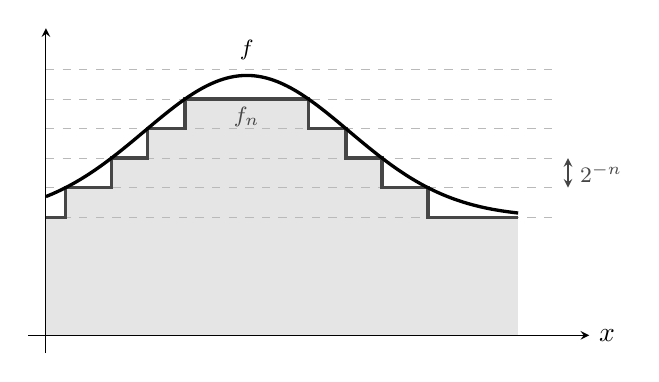
\begin{tikzpicture}[scale=1.5,>=stealth]
    % staircase below f
    \fill[gray!20] (0,0) rectangle (0.166,1.00);
    \fill[gray!20] (0.166,0) rectangle (0.554,1.25);
    \fill[gray!20] (0.554,0) rectangle (0.860,1.50);
    \fill[gray!20] (0.860,0) rectangle (1.177,1.75);
    \fill[gray!20] (1.177,0) rectangle (2.223,2.00);
    \fill[gray!20] (2.223,0) rectangle (2.540,1.75);
    \fill[gray!20] (2.540,0) rectangle (2.846,1.50);
    \fill[gray!20] (2.846,0) rectangle (3.234,1.25);
    \fill[gray!20] (3.234,0) rectangle (4.0,1.00);
    \draw[gray!55,dashed] (0,1.00) -- (4.3,1.00);
    \draw[gray!55,dashed] (0,1.25) -- (4.3,1.25);
    \draw[gray!55,dashed] (0,1.50) -- (4.3,1.50);
    \draw[gray!55,dashed] (0,1.75) -- (4.3,1.75);
    \draw[gray!55,dashed] (0,2.00) -- (4.3,2.00);
    \draw[gray!55,dashed] (0,2.25) -- (4.3,2.25);
    \draw[very thick,gray!55!black]
      (0,1.00) -- (0.166,1.00) -- (0.166,1.25) -- (0.554,1.25) -- (0.554,1.50)
      -- (0.860,1.50) -- (0.860,1.75) -- (1.177,1.75) -- (1.177,2.00)
      -- (2.223,2.00) -- (2.223,1.75) -- (2.540,1.75) -- (2.540,1.50)
      -- (2.846,1.50) -- (2.846,1.25) -- (3.234,1.25) -- (3.234,1.00)
      -- (4.0,1.00);
    \draw[->] (-0.15,0) -- (4.6,0) node[right] {$x$};
    \draw[->] (0,-0.15) -- (0,2.6);
    \draw[very thick,domain=0:4,samples=140,smooth]
      plot (\x,{1+1.2*exp(-(\x-1.7)*(\x-1.7)/1.5)});
    \node at (1.70,2.42) {\footnotesize $f$};
    \node[gray!55!black] at (1.70,1.85) {\footnotesize $f_{n}$};
    \draw[<->,gray!55!black] (4.42,1.25) -- (4.42,1.50);
    \node[right,gray!55!black] at (4.44,1.375) {\footnotesize $2^{-n}$};
  \end{tikzpicture}
\end{figure}

\medskip
The staircase takes, at each point, the largest multiple of $2^{-n}$ below $f$; every
halving of the mesh inserts a new level between two old ones, so the staircase can
only rise, and it rises to $f$. The picture also explains the cut-off at $2^{n}$: a
fonction étagée takes finitely many values and cannot follow $f$ up to $+\infty$, so
the construction truncates and lets the truncation level escape with $n$.

\subsection{Linéarité}

\begin{theorem}[Linéarité]
  Soit $f$ et $g$ des fonctions mesurables de $\Omega$ vers $\bar{\reals}$ dont les
  intégrales sont bien définies. On a :
  \[
    \forall \alpha \in \reals, \qquad
    \int \alpha f \, d\mu = \alpha \int f \, d\mu ,
  \]
  et
  \[
    \int (f + g) \, d\mu = \int f \, d\mu + \int g \, d\mu ,
  \]
  cette dernière égalité étant satisfaite dès que les fonctions $f$ et $g$ sont
  positives ou que l'une d'entre elles est intégrable.
\end{theorem}

\begin{proof}
  On montre successivement les deux propriétés, each by the same ladder: étagée
  positive, then mesurable positive by convergence monotone, then arbitrary sign by
  splitting into positive and negative parts.\\

  \textbf{Homogeneity.} Soit $\alpha \geq 0$. Si $f = \sum_{i=1}^{n} \alpha_{i}
  \indic_{A_{i}}$ est étagée positive, où les ensembles $A_{1},\ldots,A_{n}$ forment
  une partition de $\Omega$, la fonction $\alpha f$ est étagée positive, de sorte
  que $\int \alpha f \, d\mu = \sum_{i} \alpha \alpha_{i} \mu(A_{i}) = \alpha \int f
  \, d\mu$. Si la fonction $f$ est mesurable positive, on considère une suite
  croissante de fonctions étagées positives $(f_{n})$ qui tend vers $f$. Alors
  $(\alpha f_{n})$ est une suite croissante de fonctions étagées positives qui tend
  vers $\alpha f$, and the lemme de convergence monotone gives
  \[
    \int \alpha f \, d\mu = \lim_{n} \uparrow \int \alpha f_{n} \, d\mu
    = \alpha \lim_{n} \uparrow \int f_{n} \, d\mu = \alpha \int f \, d\mu .
  \]
  Si $f$ est une fonction mesurable, d'intégrale bien définie, on applique le
  résultat précédent aux fonctions $(\alpha f)^{+} = \alpha f^{+}$ et $(\alpha
  f)^{-} = \alpha f^{-}$; negative $\alpha$ then follows from the sign-reversal
  proposition.\\

  \textbf{Additivity.} On considère tout d'abord le cas où les fonctions $f$ et $g$
  sont étagées positives. On écrit :
  \[
    f = \sum_{i=1}^{n} \alpha_{i} \indic_{A_{i}}
    \qquad \text{and} \qquad
    g = \sum_{j=1}^{m} \beta_{j} \indic_{B_{j}},
  \]
  où les ensembles $A_{1},\ldots,A_{n}$ et $B_{1},\ldots,B_{m}$ forment des
  partitions de $\Omega$. La fonction $f + g$ est étagée positive, avec :
  \[
    f + g = \sum_{i=1}^{n} \sum_{j=1}^{m} (\alpha_{i} + \beta_{j})
      \indic_{A_{i} \intersect B_{j}} ,
  \]
  and therefore, on obtient :
  \begin{align*}
    \int (f+g) \, d\mu
      &= \sum_{i=1}^{n} \sum_{j=1}^{m} (\alpha_{i} + \beta_{j})
         \mu(A_{i} \intersect B_{j}) \\
      &= \sum_{i=1}^{n} \sum_{j=1}^{m} \alpha_{i} \mu(A_{i} \intersect B_{j})
       + \sum_{i=1}^{n} \sum_{j=1}^{m} \beta_{j} \mu(A_{i} \intersect B_{j}) \\
      &= \sum_{i=1}^{n} \alpha_{i} \mu(A_{i}) + \sum_{j=1}^{m} \beta_{j} \mu(B_{j})
       = \int f \, d\mu + \int g \, d\mu .
  \end{align*}
  Si $f$ et $g$ sont mesurables positives, on considère des suites croissantes de
  fonctions étagées positives $(f_{n})$ et $(g_{n})$ qui tendent respectivement vers
  $f$ et $g$. Alors $(f_{n} + g_{n})$ est une suite croissante de fonctions étagées
  positives qui tend vers $f+g$, and the lemme de convergence monotone gives $\int
  (f+g) \, d\mu = \lim_{n} \uparrow ( \int f_{n} \, d\mu + \int g_{n} \, d\mu ) =
  \int f \, d\mu + \int g \, d\mu$.

  Finally, si $f$ ou $g$ est intégrable,
  \[
    \int (f+g)^{+} \, d\mu \leq \int (f^{+} + g^{+}) \, d\mu
    = \int f^{+} \, d\mu + \int g^{+} \, d\mu < \infty
  \]
  ou
  \[
    \int (f+g)^{-} \, d\mu \leq \int (f^{-} + g^{-}) \, d\mu
    = \int f^{-} \, d\mu + \int g^{-} \, d\mu < \infty ,
  \]
  l'intégrale de $f+g$ est donc bien définie. Comme :
  \[
    f + g = (f+g)^{+} - (f+g)^{-} = f^{+} - f^{-} + g^{+} - g^{-}
  \]
  on a :
  \[
    (f+g)^{+} + f^{-} + g^{-} = (f+g)^{-} + f^{+} + g^{+} ,
  \]
  ces fonctions étant positives, the positive case applies to this identity:
  \[
    \int (f+g)^{+} \, d\mu + \int f^{-} \, d\mu + \int g^{-} \, d\mu
    = \int (f+g)^{-} \, d\mu + \int f^{+} \, d\mu + \int g^{+} \, d\mu ,
  \]
  and rearranging gives $\int (f+g) \, d\mu = \int f \, d\mu + \int g \, d\mu$.
\end{proof}

\begin{remark}[Rearranging into positive parts, and why]
  The last step is the only subtle one. One cannot simply subtract $\int f^{-}$ from
  both sides of an equality between possibly infinite quantities; the rearrangement
  into an identity between \emph{positive} functions is what allows the additive case
  already proved to be applied, and the hypothesis that one of $f$, $g$ is integrable
  is what guarantees that the terms being moved are finite. Drop that hypothesis and
  the statement fails: with $f = \indic_{\reals_{+}}$ and $g = -\indic_{\reals_{+}}$
  the left-hand side is $0$ while the right-hand side is $\infty - \infty$.
\end{remark}

\begin{remark}[The three-stage method]
  The proof just given is the pattern of the whole chapter. A statement about the
  integral is proved first for fonctions étagées positives, where it is a finite
  sum; then for positive mesurable functions, by taking an increasing sequence of
  fonctions étagées and applying the lemme de convergence monotone on each side; then
  for mesurable functions of arbitrary sign, by applying the positive case to $f^{+}$
  and to $f^{-}$ and subtracting, which needs one of the two to be finite. Every
  proof below that begins ``by the three-stage method'' is this argument, and only
  its first stage is ever written out.
\end{remark}

\begin{remark}[The order of the chapter is not circular]
  It looks as though linearity has just been proved using convergence monotone, while
  convergence monotone is stated as a theorem only two subsections below. It is not
  circular, and the point is worth stating once, being the single most confusing
  thing in this chapter. What linearity uses is the \emph{lemma} form: an
  \emph{everywhere} increasing sequence of positive mesurable functions with
  everywhere pointwise limit. That lemma was proved directly from the definition of
  the integral as a supremum over fonctions étagées, using only monotonicity and
  continuity from below of the mesure, and no linearity whatsoever. The
  \emph{theorem} form below weakens the hypothesis to convergence \textit{presque
  partout}, and its proof restricts to the set where convergence holds and invokes
  the lemma there --- and that restriction is where linearity and the results on
  ensembles négligeables are needed. The dependency runs lemma $\to$ linearity $\to$
  ensembles négligeables $\to$ theorem, with no cycle, and these notes keep that
  order.
\end{remark}

\begin{corollary}[L'intégrabilité se lit sur le module]
  Une fonction mesurable $f$ est intégrable si et seulement si $\int |f| \, d\mu <
  \infty$.
\end{corollary}

\begin{proof}
  Comme $|f| = f^{+} + f^{-}$, on a par linéarité de l'intégrale, in the positive
  case :
  \[
    \int |f| \, d\mu = \int f^{+} \, d\mu + \int f^{-} \, d\mu ,
  \]
  qui est finie si et seulement si $\int f^{+} \, d\mu < \infty$ et $\int f^{-} \,
  d\mu < \infty$, that is, if and only if $f$ is integrable.
\end{proof}

\begin{corollary}[Additivité dénombrable de l'intégrale]
  Pour toute suite de fonctions mesurables positives $(f_{n})_{n \geq 1}$,
  \[
    \sum_{n \geq 1} \int f_{n} \, d\mu = \int \left( \sum_{n \geq 1} f_{n} \right)
      d\mu .
  \]
\end{corollary}

\begin{proof}
  La suite $\left( \sum_{n=1}^{k} f_{n} \right)_{k \geq 1}$ (the partial sums) est
  une suite croissante de fonctions mesurables positives qui tend vers $f = \sum_{n
  \geq 1} f_{n}$, so the lemme de convergence monotone gives
  \[
    \lim_{k} \uparrow \int \sum_{n=1}^{k} f_{n} \, d\mu = \int f \, d\mu ,
  \]
  while, par ailleurs, la linéarité de l'intégrale implique que
  \[
    \lim_{k} \uparrow \int \sum_{n=1}^{k} f_{n} \, d\mu
    = \lim_{k} \uparrow \sum_{n=1}^{k} \int f_{n} \, d\mu
    = \sum_{n \geq 1} \int f_{n} \, d\mu . \qedhere
  \]
\end{proof}

\begin{remark}[Positivity is the whole hypothesis]
  Nothing is assumed about convergence: both sides may be $+\infty$, and the corollary
  asserts that they are infinite together. This is the interchange of a sum and an
  integral that costs nothing; it is used below to prove that a mesure à densité is a
  mesure, and again inside the construction of the mesure produit. Without
  positivity the interchange needs domination.
\end{remark}

\subsection{Ensembles négligeables}

On rappelle qu'un ensemble $A \in \mathcal{F}$ est dit négligeable si $\mu(A) = 0$,
as in the previous chapter.

\begin{prop}[Intégrale sur un ensemble négligeable]
  Soit $f : \Omega \to \reals$ une fonction mesurable et $A$ un ensemble négligeable.
  Alors
  \[
    \int_{A} f \, d\mu = 0 .
  \]
\end{prop}

\begin{proof}
  By the three-stage method. Si $f = \sum_{i=1}^{n} \alpha_{i} \indic_{A_{i}}$ est
  étagée positive, alors la fonction $f \indic_{A} = \sum_{i=1}^{n} \alpha_{i}
  \indic_{A_{i} \intersect A}$ est elle-même étagée positive. On en déduit :
  \[
    \int_{A} f \, d\mu = \sum_{i=1}^{n} \alpha_{i} \mu(A_{i} \intersect A)
    \leq \sum_{i=1}^{n} \alpha_{i} \mu(A) = 0 .
  \]
  The two remaining stages use $(f \indic_{A})^{+} = f^{+} \indic_{A}$ and $(f
  \indic_{A})^{-} = f^{-} \indic_{A}$.
\end{proof}

On rappelle qu'une propriété est vraie ``presque partout'' (ce que l'on note p.p.) si
sa négation correspond à un ensemble négligeable, and that the mesure it refers to is
always the one the integral is taken against.

\begin{theorem}[L'intégrale ne voit pas les ensembles négligeables]
  Soit $f, g : \Omega \to \reals$ des fonctions mesurables. Alors
  \begin{enumerate}
    \item $f = 0$ p.p. implique $\int f \, d\mu = 0$ ;
    \item $f = g$ p.p. implique $\int f \, d\mu = \int g \, d\mu$ dès que l'une de
      ces intégrales existe ;
    \item $f \geq 0$ p.p. implique $\int f \, d\mu \geq 0$ ; si de plus $\int f \,
      d\mu = 0$ alors $f = 0$ p.p. ;
    \item $f \leq g$ p.p. implique $\int f \, d\mu \leq \int g \, d\mu$ dès que ces
      intégrales existent ; si de plus $\int f \, d\mu = \int g \, d\mu < \infty$
      alors $f = g$ p.p.
  \end{enumerate}
\end{theorem}

\begin{proof}
  \textbf{1.} L'ensemble $A = \{f \neq 0\}$ est négligeable. Comme $f = f
  \indic_{A}$, on a par la proposition précédente $\int f \, d\mu = \int_{A} f \,
  d\mu = 0$.\\

  \textbf{2.} Si $f, g$ sont positives, on note $A = \{f = g\}$, whose complement is
  négligeable. Comme $f = f \indic_{A} + f \indic_{A^{c}}$, and likewise for $g$, on
  a par linéarité et par la proposition précédente $\int f \, d\mu = \int f
  \indic_{A} \, d\mu = \int g \indic_{A} \, d\mu = \int g \, d\mu$. In general $f^{+}
  = g^{+}$ p.p. et $f^{-} = g^{-}$ p.p., so the positive case applies to each; if
  one of the two integrals is well defined, so is the other, and they are equal.\\

  \textbf{3.} On définit $A = \{f \geq 0\}$. Comme $f = f \indic_{A}$ p.p., on a par
  le résultat précédent $\int f \, d\mu \geq 0$. Si de plus $\int f \, d\mu = 0$, on
  définit $A_{n} = \{f \geq \frac{1}{n}\}$. Comme $f \indic_{A_{n}} \leq f
  \indic_{A}$,
  \[
    \int f \, d\mu \geq \int f \indic_{A_{n}} \, d\mu
    \geq \frac{1}{n} \mu(A_{n}) ,
  \]
  on a donc $\mu(A_{n}) = 0$ pour tout $n$, et comme $A_{n} \uparrow \{f > 0\}$,
  continuity from below gives $\mu(\{f > 0\}) = 0$. On en déduit que $f = 0$ p.p.\\

  \textbf{4.} Soit $A = \{f \leq g\}$, whose complement is négligeable. Comme $f
  \indic_{A} \leq g \indic_{A}$, on a $\int f \, d\mu \leq \int g \, d\mu$ by the
  second point. Si de plus $\int f \, d\mu = \int g \, d\mu < \infty$, alors $g - f
  \geq 0$ p.p. avec $\int (g-f) \, d\mu = 0$, ce qui implique $f = g$ p.p. d'après le
  résultat précédent.
\end{proof}

\begin{remark}[Finiteness in the last statement]
  The finiteness $\int f \, d\mu = \int g \, d\mu < \infty$ in the fourth point is
  not decoration. It is what makes $\int (g-f) \, d\mu = 0$ legitimate: subtracting
  two infinite integrals says nothing. Take $f = \indic_{\reals_{+}}$ and $g =
  \indic_{\reals}$ against $\lambda$. Both integrals are defined and equal to
  $+\infty$, and $f \leq g$ everywhere, yet $f$ and $g$ differ on the whole of
  $]-\infty,0[$, which is very far from négligeable. Equal infinite integrals say
  nothing about the two functions; only equal finite ones do. The same remark applies
  to the equality case of the third point, where the hypothesis is the value $0$,
  which is finite by construction.
\end{remark}

\begin{theorem}[Une fonction intégrable est p.p. finie]
  Toute fonction intégrable est p.p. finie.
\end{theorem}

\begin{proof}
  Soit $f$ une fonction positive intégrable. Notons $A = \{f = +\infty\}$. Pour tout
  $n \geq 1$, $f \geq f_{n}$ avec $f_{n} = n \indic_{A}$. On en déduit :
  \[
    \int f \, d\mu \geq \int f_{n} \, d\mu = n \mu(A) .
  \]
  Si $\mu(A) > 0$ alors, en faisant tendre $n \to +\infty$, on obtient $\int f \,
  d\mu = +\infty$, une contradiction. L'ensemble $A$ est donc négligeable, ce qui
  signifie que $f$ est p.p. finie. Si $f$ est intégrable (of arbitrary sign), alors
  $\int f^{+} \, d\mu < \infty$ et $\int f^{-} \, d\mu < \infty$. D'après le
  résultat précédent, $f^{+}$ et $f^{-}$ sont p.p. finies, ce qui veut dire que $f$
  est p.p. finie.
\end{proof}

\subsection{Convergence monotone, convergence dominée}

This is where the intégrale de Lebesgue earns its place. Two theorems give
conditions under which a limit may be taken inside an integral, and a lemma sits
between them providing an inequality that always holds.

\begin{theorem}[Convergence monotone]
  Soit $f$ une fonction mesurable et $(f_{n})_{n \geq 1}$ une suite croissante de
  fonctions mesurables positives qui converge p.p. vers $f$. Alors :
  \[
    \lim_{n} \int f_{n} \, d\mu = \int f \, d\mu .
  \]
\end{theorem}

\begin{proof}
  Soit $A = \{\lim_{n} f_{n} = f\}$ l'ensemble des points où il y a convergence. Its
  complement is négligeable, so by the lemme de convergence monotone applied to the
  sequence $(f_{n} \indic_{A})$, which increases to $f \indic_{A}$ everywhere,
  \[
    \lim_{n} \int f_{n} \, d\mu = \lim_{n} \int f_{n} \indic_{A} \, d\mu
    = \int f \indic_{A} \, d\mu = \int f \, d\mu ,
  \]
  the first and last equalities being the theorem on ensembles négligeables just
  proved.
\end{proof}

\begin{remark}[The theorem is the lemma, plus p.p.]
  The only thing added to the lemma is the tolerance of a négligeable exceptional
  set, and the proof is the restriction to $A$ that the non-circularity remark above
  anticipated. It is the form one actually applies, because hypotheses in practice
  hold only p.p.
\end{remark}

Le théorème de convergence dominée repose sur le résultat suivant.

\begin{lemma}[Lemme de Fatou (\textit{Fatou's lemma})]
  Pour toute suite $(f_{n})_{n \geq 1}$ de fonctions mesurables positives,
  \[
    \int \liminf_{n} f_{n} \, d\mu \leq \liminf_{n} \int f_{n} \, d\mu .
  \]
\end{lemma}

\begin{proof}
  The sequence $( \inf_{k \geq n} f_{k} )_{n \geq 1}$ is increasing and positive with
  limit $\liminf_{n} f_{n}$, so par convergence monotone, $\int \liminf_{n} f_{n} \,
  d\mu = \lim_{n} \int \inf_{k \geq n} f_{k} \, d\mu$. Comme $\inf_{k \geq n} f_{k}
  \leq f_{k}$ pour tout $k \geq n$, monotonicity gives $\int \inf_{k \geq n} f_{k}
  \, d\mu \leq \inf_{k \geq n} \int f_{k} \, d\mu$, et par passage à la limite,
  $\int \liminf_{n} f_{n} \, d\mu \leq \liminf_{n} \int f_{n} \, d\mu$.
\end{proof}

\begin{remark}[Fatou gives an inequality and nothing more]
  Le lemme de Fatou fournit uniquement une inégalité, which can be strict. Appliqué
  aux fonctions $f_{n} = \indic_{[n,+\infty[}$, against the mesure de Lebesgue, on a
  $\liminf_{n} f_{n} = 0$, si bien que
  \[
    \int \liminf_{n} f_{n} \, d\lambda = 0 ,
    \qquad \text{while} \qquad
    \liminf_{n} \int f_{n} \, d\lambda = +\infty .
  \]
  Mass escaping to infinity is lost in the limit but not in the integrals, and the
  inequality records exactly that loss.
\end{remark}

\begin{theorem}[Convergence dominée (\textit{dominated convergence})]
  Soit $f$ une fonction mesurable et $(f_{n})_{n \geq 1}$ une suite de fonctions
  mesurables qui converge p.p. vers $f$. S'il existe une fonction \emph{intégrable}
  $g$ telle que $|f_{n}| \leq g$ pour tout $n \geq 1$, alors la fonction $f$ est
  intégrable et
  \[
    \lim_{n} \int f_{n} \, d\mu = \int f \, d\mu .
  \]
\end{theorem}

\begin{proof}
  Le lemme de Fatou, applied to $(|f_{n}|)$, implique que
  \[
    \int |f| \, d\mu = \int \liminf_{n} |f_{n}| \, d\mu
    \leq \liminf_{n} \int |f_{n}| \, d\mu \leq \int g \, d\mu < \infty ,
  \]
  de sorte que la fonction $f$ est intégrable. Les fonctions $g - f_{n}$ et $g +
  f_{n}$ étant mesurables positives pour tout $n$, le lemme de Fatou, applied to each
  of the two sequences, implique également que :
  \begin{align*}
    \int g \, d\mu - \int f \, d\mu &= \int (g - f) \, d\mu
      \leq \liminf_{n} \int (g - f_{n}) \, d\mu
      = \int g \, d\mu - \limsup_{n} \int f_{n} \, d\mu , \\
    \int g \, d\mu + \int f \, d\mu &= \int (g + f) \, d\mu
      \leq \liminf_{n} \int (g + f_{n}) \, d\mu
      = \int g \, d\mu + \liminf_{n} \int f_{n} \, d\mu .
  \end{align*}
  Since $\int g \, d\mu$ is finite it can be cancelled from both lines, and on tire de
  ces inégalités que
  \[
    \int f \, d\mu \leq \liminf_{n} \int f_{n} \, d\mu
    \leq \limsup_{n} \int f_{n} \, d\mu \leq \int f \, d\mu ,
  \]
  d'où l'on conclut que la suite $\int f_{n} \, d\mu$ converge vers $\int f \,
  d\mu$.
\end{proof}

\begin{remark}[Where the domination is spent]
  The function $g$ is used three times: to make $f$ integrable, to make $g - f_{n}$
  and $g + f_{n}$ positive so that Fatou applies, and --- decisively --- to allow
  $\int g \, d\mu$ to be cancelled from both sides. That cancellation is illegal if
  $\int g \, d\mu = +\infty$, which is why the hypothesis is not that some function
  dominates the sequence but that an \emph{integrable} one does, and one that works
  for every $n$ simultaneously.
\end{remark}

\begin{example}[Domination cannot be dropped]
  Let $f_{n} = n \indic_{]0,1/n[}$ on $\reals$ with the mesure de Lebesgue. For every
  $x$, $f_{n}(x) \to 0$: a fixed $x > 0$ leaves the interval as soon as $n > 1/x$,
  and $f_{n}(x) = 0$ for $x \leq 0$ throughout. Yet
  \[
    \int f_{n} \, d\lambda = n \cdot \frac{1}{n} = 1
    \qquad \text{for every } n, \qquad \text{while} \qquad
    \int \lim_{n} f_{n} \, d\lambda = 0 .
  \]
  The limit and the integral cannot be exchanged. Any function dominating the whole
  sequence is at least the pointwise supremum $\sup_{n} f_{n}$, the staircase equal
  to $k$ on $]\frac{1}{k+1},\frac{1}{k}[$; it therefore exceeds $x \mapsto 1/x - 1$
  on $]0,1[$, whose integral diverges. No integrable dominating function exists ---
  exactly as the theorem requires. Note
  that Fatou's inequality is satisfied, $0 \leq 1$, as it must be.
\end{example}

\begin{figure}[h!]
  \centering
  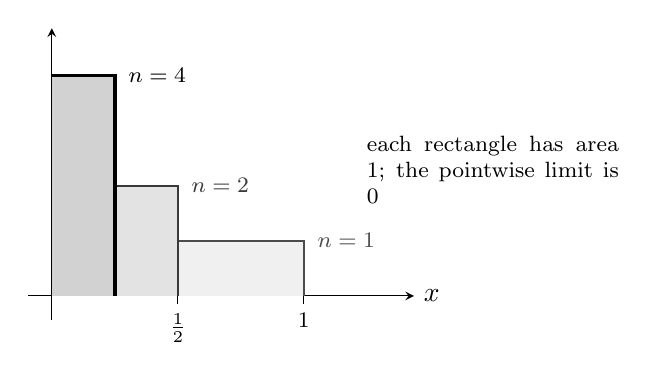
\begin{tikzpicture}[scale=1.0,>=stealth]
    \draw[->] (-0.3,0) -- (4.6,0) node[right] {$x$};
    \draw[->] (0,-0.3) -- (0,3.4);
    % n = 1
    \fill[gray!12] (0,0) rectangle (3.2,0.7);
    \draw[thick,gray!60!black] (0,0.7) -- (3.2,0.7) -- (3.2,0);
    \node[right,gray!60!black] at (3.25,0.7) {\footnotesize $n=1$};
    % n = 2
    \fill[gray!22] (0,0) rectangle (1.6,1.4);
    \draw[thick,gray!45!black] (0,1.4) -- (1.6,1.4) -- (1.6,0);
    \node[right,gray!45!black] at (1.65,1.4) {\footnotesize $n=2$};
    % n = 4
    \fill[gray!35] (0,0) rectangle (0.8,2.8);
    \draw[very thick] (0,2.8) -- (0.8,2.8) -- (0.8,0);
    \node[right] at (0.85,2.8) {\footnotesize $n=4$};
    \draw (3.2,0) -- (3.2,-0.1) node[below] {\footnotesize $1$};
    \draw (1.6,0) -- (1.6,-0.1) node[below] {\footnotesize $\frac{1}{2}$};
    \node at (5.6,1.6) {\parbox{3.2cm}{\footnotesize each rectangle has area
      $1$; the pointwise limit is $0$}};
  \end{tikzpicture}
\end{figure}

\medskip
The picture is the whole counter-example: a rectangle of area $1$ that becomes
taller and narrower without ever losing mass, while at every fixed $x$ it eventually
disappears. Mass escapes upwards here, as it escaped sideways in the Fatou remark,
and an integrable dominating function is precisely a ceiling that forbids both.

\subsection{Lien avec l'intégrale de Riemann}

Nous montrons ici que l'intégrale de Lebesgue généralise l'intégrale de Riemann. On
se donne un intervalle $[a,b]$ de $\reals$ avec $a < b$.

\begin{definition}[Fonction en escalier (\textit{step function})]
  Une fonction $f : [a,b] \to \reals$ est dite \textbf{en escalier} s'il existe une
  subdivision $a = x_{0} < x_{1} < \ldots < x_{n} = b$ de l'intervalle $[a,b]$ telle
  que $f$ est constante sur chaque intervalle $]x_{0},x_{1}[, \ldots,
  ]x_{n-1},x_{n}[$.
\end{definition}

L'intégrale de Riemann d'une fonction en escalier $f$ est définie par :
\[
  \int_{a}^{b} f(x) \, dx = \sum_{i=0}^{n-1} \alpha_{i} (x_{i+1} - x_{i}) ,
\]
où $\alpha_{0},\ldots,\alpha_{n-1}$ sont les valeurs prises par $f$ sur les
intervalles respectifs $]x_{0},x_{1}[, \ldots, ]x_{n-1},x_{n}[$. La fonction $f$
étant étagée in the sense of this chapter, on vérifie aisément que c'est également
l'intégrale de Lebesgue par rapport à la mesure de Lebesgue :
\[
  \int_{[a,b]} f \, d\lambda = \sum_{i=0}^{n-1} \alpha_{i}
    \lambda(]x_{i},x_{i+1}[) = \int_{a}^{b} f(x) \, dx .
\]
A fonction en escalier is the elementary brick of the Riemann theory exactly as a
fonction étagée is of the Lebesgue theory; the difference is that a fonction en
escalier is constant on \emph{intervals} while a fonction étagée is constant on
arbitrary mesurable sets, and that single relaxation is the whole gap between the
two theories.

\begin{definition}[Intégrale de Riemann (\textit{Riemann integral})]
  Une fonction bornée $f : [a,b] \to \reals$ est \textbf{intégrable au sens de
  Riemann} (\textit{Riemann-integrable}) si :
  \[
    \sup \left\{ \int_{a}^{b} g(x) \, dx : g \leq f, \; g \text{ a step function}
    \right\}
    = \inf \left\{ \int_{a}^{b} h(x) \, dx : f \leq h, \; h \text{ a step function}
    \right\} ,
  \]
  cette valeur étant son intégrale, notée $\int_{a}^{b} f(x) \, dx$.
\end{definition}

\begin{theorem}[Intégrable au sens de Riemann implique intégrable au sens de Lebesgue]
  Une fonction $f : [a,b] \to \reals$ intégrable au sens de Riemann a une intégrale
  par rapport à la mesure de Lebesgue et les deux intégrales coïncident :
  \[
    \int_{a}^{b} f(x) \, dx = \int_{[a,b]} f \, d\lambda .
  \]
\end{theorem}

\begin{proof}
  Soit $(g_{n})_{n \geq 1}$ une suite croissante de fonctions en escalier telle que
  $g_{n} \leq f$ pour tout $n$ et :
  \[
    \lim_{n} \int_{a}^{b} g_{n}(x) \, dx = \int_{a}^{b} f(x) \, dx ,
  \]
  et de même, soit $(h_{n})_{n \geq 1}$ une suite décroissante de fonctions en
  escalier telle que $h_{n} \geq f$ pour tout $n$ et :
  \[
    \lim_{n} \int_{a}^{b} h_{n}(x) \, dx = \int_{a}^{b} f(x) \, dx ;
  \]
  both exist by the definition of a fonction intégrable au sens de Riemann, replacing
  a maximising sequence by the running maximum of its terms in the first case and
  the running minimum in the second. Les limites respectives $g$ et $h$ de ces suites
  sont mesurables et bornées, $f$ being bounded, de sorte que, par convergence
  dominée --- the constant bound being integrable on the bounded interval $[a,b]$
  --- both limits of intégrales de Riemann are intégrales de Lebesgue. On a donc :
  \[
    \int_{[a,b]} g \, d\lambda = \int_{a}^{b} f(x) \, dx
    = \int_{[a,b]} h \, d\lambda .
  \]
  Comme $g \leq f \leq h$, the equality case in the theorem on ensembles négligeables
  gives $g = h$ p.p., et donc $g = f = h$ p.p., ce qui implique $\int_{a}^{b} f(x) \,
  dx = \int_{[a,b]} f \, d\lambda$.
\end{proof}

\begin{remark}[Which tribu the Riemann theory really uses]
  Le théorème suggère que toute fonction intégrable au sens de Riemann est mesurable
  pour la tribu de Borel. Ce n'est pas le cas. Elle est mesurable par rapport à la
  \textbf{tribu de Lebesgue} (\textit{Lebesgue $\sigma$-algebra}), définie comme la
  tribu de Borel complétée de tous les ensembles négligeables pour la mesure de
  Lebesgue (ensembles mesurables négligeables et leurs sous-ensembles). Ce détail
  technique ne change rien en pratique, l'intégrale de Lebesgue étant définie de la
  même manière sur la tribu complétée; what the proof above shows is that $f$ agrees
  p.p. with the Borel function $g$.
\end{remark}

Il reste à étendre le résultat aux intégrales impropres. Soit $a, b \in \bar{\reals}$.
Pour toute fonction $f$ localement intégrable au sens de Riemann sur $]a,b[$
(c'est-à-dire dont l'intégrale de Riemann est définie sur tout compact de $]a,b[$),
on définit l'intégrale de Riemann comme la limite lorsqu'elle existe des intégrales
\[
  \int_{a_{n}}^{b_{n}} f(x) \, dx
\]
pour toutes suites $(a_{n})_{n \geq 1}$ et $(b_{n})_{n \geq 1}$ respectivement
strictement décroissante et strictement croissante, de limites $a$ et $b$. On note
toujours cette intégrale $\int_{a}^{b} f(x) \, dx$.

\begin{theorem}[Intégrale de Riemann impropre d'une fonction intégrable]
  Soit $a, b \in \bar{\reals}$ et $f$ une fonction localement intégrable au sens de
  Riemann sur $]a,b[$, avec
  \[
    \int_{a}^{b} |f(x)| \, dx < \infty .
  \]
  Alors :
  \[
    \int_{a}^{b} f(x) \, dx = \int_{[a,b]} f \, d\lambda .
  \]
\end{theorem}

\begin{proof}
  Soit $(a_{n})$ et $(b_{n})$ des suites as above. Par le théorème précédent,
  $\int_{a_{n}}^{b_{n}} |f(x)| \, dx = \int_{[a_{n},b_{n}]} |f| \, d\lambda$ pour
  tout $n$. The functions $|f| \indic_{[a_{n},b_{n}]}$ increase to $|f|
  \indic_{[a,b]}$, so par convergence monotone,
  \[
    \int_{[a,b]} |f| \, d\lambda = \lim_{n} \int_{a_{n}}^{b_{n}} |f(x)| \, dx
    = \int_{a}^{b} |f(x)| \, dx < \infty ,
  \]
  which says that $f$ is Lebesgue-integrable on $[a,b]$. The functions $f
  \indic_{[a_{n},b_{n}]}$ are then dominated by the integrable $|f| \indic_{[a,b]}$
  and converge pointwise to $f \indic_{[a,b]}$, so par convergence dominée, on en
  déduit que $\int_{a}^{b} f(x) \, dx = \int_{[a,b]} f \, d\lambda$.
\end{proof}

\begin{remark}[The hypothesis is absolute integrability, and it is the point]
  Le théorème exige que la fonction soit intégrable, that is $\int_{a}^{b} |f(x)| \,
  dx < \infty$, and not merely that it have a convergent improper integral. Ainsi
  l'intégrale impropre
  \[
    \int_{-\infty}^{+\infty} \frac{\sin x}{x} \, dx
  \]
  est définie au sens de Riemann --- the positive and negative humps cancel in the
  limit, and the value is $\pi$ --- mais pas au sens de Lebesgue, since $\int |\sin
  x / x| \, dx = +\infty$ and the Lebesgue definition subtracts two infinite parts.
  This is the one place where the Riemann theory reaches something the Lebesgue
  theory does not, and the reason is structural: the intégrale de Lebesgue is
  absolute by construction, since it is built from $f^{+}$ and $f^{-}$ separately,
  while an intégrale de Riemann impropre is a limit of symmetric truncations and can
  exploit cancellation.
\end{remark}

\begin{remark}[The converse fails in the other direction too]
  Not every Lebesgue-integrable function is intégrable au sens de Riemann. The
  function $\indic_{\mathbb{Q}}$ on $[0,1]$ has intégrale de Lebesgue $0$, while
  every fonction en escalier below it is $\leq 0$ and every fonction en escalier
  above it is $\geq 1$ on each subinterval, so the lower Riemann sums are $\leq 0$,
  the upper ones $\geq 1$, and the two do not meet. Taken with the previous remark,
  the picture is: the two classes of functions overlap but neither contains the
  other, and where they overlap the two integrals agree.
\end{remark}

Comme l'intégrale de Riemann correspond à une intégrale par rapport à la mesure de
Lebesgue, on utilisera les notations
\[
  \int_{a}^{b} f(x) \, dx
  \qquad \text{and} \qquad
  \int_{[a,b]} f \, d\lambda
\]
indifféremment. Les résultats classiques de l'intégrale comme le théorème fondamental de l'analyse
ou l'intégration par parties s'appliquent à l'intégrale de Lebesgue, par rapport à
la mesure de Lebesgue. Tous ces résultats s'étendent aux fonctions de $n$ variables,
sur l'ensemble $\reals^{n}$ muni de la tribu de Borel.

\subsection{Mesures discrètes}

The integral has been defined against an arbitrary mesure. It is time to see what it
becomes for the two mesures the previous chapter singled out. Against the mesure de
Lebesgue it is the classical integral, as the preceding subsection showed. Nous
allons maintenant caractériser l'intégrale de Lebesgue par rapport à une mesure
discrète: it is a sum --- which is what makes chapter 1, where probabilities were
sums over a countable set, a special case of the theory being built here rather than
a separate subject. The bridge is the following pair of results.

\begin{prop}[Mesure somme]
  Soit $(\mu_{i})_{i \in I}$ une famille de mesures sur $(\Omega,\mathcal{F})$.
  L'intégrale d'une fonction mesurable $f : \Omega \to \bar{\reals}$ par rapport à la
  \textbf{mesure somme} (\textit{sum measure}) $\mu = \sum_{i \in I} \mu_{i}$ est
  donnée par
  \[
    \int f \, d\mu = \sum_{i \in I} \int f \, d\mu_{i} ,
  \]
  si cette intégrale est bien définie, c'est-à-dire si :
  \[
    \sum_{i \in I} \int f^{+} \, d\mu_{i} < \infty
    \qquad \text{or} \qquad
    \sum_{i \in I} \int f^{-} \, d\mu_{i} < \infty .
  \]
\end{prop}

\begin{proof}
  By the three-stage method. Si $f = \sum_{j=1}^{n} \alpha_{j} \indic_{A_{j}}$ est
  une fonction étagée positive, alors
  \[
    \int f \, d\mu = \sum_{j=1}^{n} \alpha_{j} \sum_{i \in I} \mu_{i}(A_{j})
    = \sum_{i \in I} \sum_{j=1}^{n} \alpha_{j} \mu_{i}(A_{j})
    = \sum_{i \in I} \int f \, d\mu_{i} ,
  \]
  the interchange of the two sums being legitimate because all the terms are
  positive. The second stage applies the lemme de convergence monotone once to $\mu$
  and once to each $\mu_{i}$, the interchange of the limit and the sum over $I$ being
  again a matter of positive terms.
\end{proof}

L'archétype des mesures discrètes est la mesure de Dirac.

\begin{prop}[Mesure de Dirac]
  Soit $\delta_{a}$ la mesure de Dirac en $a \in \Omega$. Toute fonction mesurable
  $f : \Omega \to \bar{\reals}$ a pour intégrale :
  \[
    \int f \, d\delta_{a} = f(a) .
  \]
\end{prop}

\begin{proof}
  By the three-stage method. Si $f = \sum_{i=1}^{n} \alpha_{i} \indic_{A_{i}}$ est
  une fonction étagée positive, alors $\int f \, d\delta_{a} = \sum_{i} \alpha_{i}
  \indic_{A_{i}}(a) = f(a)$; the second stage gives $\lim_{n} f_{n}(a) = f(a)$, and
  the third $f^{+}(a) - f^{-}(a) = f(a)$.
\end{proof}

On montre de la même manière que pour toute mesure $\mu = \alpha \delta_{a}$ avec
$\alpha > 0$ et $a \in \Omega$, $\int f \, d\mu = \alpha f(a)$. Combining this with
the mesure somme, on obtient l'intégrale d'une fonction mesurable par rapport à toute
mesure discrète
\[
  \mu = \sum_{i \in I} \alpha_{i} \delta_{a_{i}} ,
\]
où $I$ est un ensemble au plus dénombrable et $\alpha_{i} > 0$, $a_{i} \in \Omega$
pour tout $i \in I$.

\begin{theorem}[L'intégrale par rapport à une mesure discrète est une somme]
  Toute fonction mesurable $f : \Omega \to \bar{\reals}$ a pour intégrale :
  \[
    \int f \, d\mu = \sum_{i \in I} \alpha_{i} f(a_{i})
  \]
  dès que
  \[
    \sum_{i \in I} \alpha_{i} f^{+}(a_{i}) < \infty
    \qquad \text{or} \qquad
    \sum_{i \in I} \alpha_{i} f^{-}(a_{i}) < \infty .
  \]
\end{theorem}

\begin{remark}[The bridge back to the discrete chapter]
  This is the statement that makes the general theory contain the discrete one. A
  discrete probability on a countable $\Omega$ is $\prob = \sum_{\omega \in \Omega}
  p(\omega) \delta_{\omega}$, and the theorem reads $\int f \, d\prob = \sum_{\omega}
  p(\omega) f(\omega)$: every espérance computed in chapter 1 as a weighted sum is
  an intégrale de Lebesgue, and every theorem proved below for the intégrale de
  Lebesgue applies verbatim to those sums. In particular the countable additivity
  corollary above is the interchange of two sums, and convergence dominée is the
  interchange of a limit and a series.
\end{remark}

\begin{example}[The mesure de comptage turns the integral into a series]
  Soit $\mu = \sum_{n \in \mathbb{N}} \delta_{n}$ la mesure de comptage de
  $\mathbb{N}$. L'intégrale d'une fonction mesurable $f : \reals \to \bar{\reals}$
  est la série
  \[
    \int f \, d\mu = \sum_{n=0}^{+\infty} f(n)
  \]
  dès que $\sum_{n=0}^{+\infty} f^{+}(n) < \infty$ ou $\sum_{n=0}^{+\infty}
  f^{-}(n) < \infty$. For $f(x) = e^{-x}$ this gives
  \[
    \int e^{-x} \, d\mu(x) = \sum_{n \geq 0} e^{-n} = \frac{1}{1 - e^{-1}}
    = \frac{e}{e-1} .
  \]
\end{example}

\begin{example}[A mesure with a discrete part and a continuous part]
  Let $\mu = \delta_{0} + \lambda$ on $\reals$. By the proposition on the mesure
  somme,
  \[
    \int_{\reals_{+}} e^{-x} \, d\mu(x)
    = \int_{\reals_{+}} e^{-x} \, d\delta_{0}(x)
      + \int_{\reals_{+}} e^{-x} \, d\lambda(x)
    = 1 + \int_{0}^{+\infty} e^{-x} \, dx = 2 .
  \]
  Nothing in the theory forbids mixing an atom and a continuous part, and lois of
  this kind appear as soon as a variable aléatoire is truncated.
\end{example}

\subsection{Mesures à densité}

Integration produces new mesures. This subsection says which ones, and when every
mesure of a given kind arises this way.

\begin{theorem}[L'intégrale d'une fonction positive définit une mesure]
  Soit $\nu$ une mesure sur $(\Omega,\mathcal{F})$ et $f$ une fonction mesurable
  positive.
  \begin{enumerate}
    \item La fonction $\mu : \mathcal{F} \to [0,+\infty]$ définie par
      \[
        \forall A \in \mathcal{F}, \qquad \mu(A) = \int_{A} f \, d\nu
      \]
      est une mesure sur $(\Omega,\mathcal{F})$.
    \item Supposons la mesure $\nu$ $\sigma$-finie. S'il existe une autre fonction
      mesurable positive $g$ telle que $\mu(A) = \int_{A} g \, d\nu$ pour tout $A \in
      \mathcal{F}$, alors $f = g$ $\nu$-p.p.
  \end{enumerate}
\end{theorem}

\begin{proof}
  \textbf{1.} On vérifie que $\mu(\emptyset) = 0$ et que pour toute famille au plus
  dénombrable $(A_{i})_{i \in I}$ d'éléments deux-à-deux disjoints,
  $\mu(\bigcup_{i} A_{i}) = \int f \sum_{i} \indic_{A_{i}} \, d\nu = \sum_{i} \int f
  \indic_{A_{i}} \, d\nu = \sum_{i} \mu(A_{i})$, the middle equality being the
  countable additivity corollary, applicable because the functions $f
  \indic_{A_{i}}$ are positive.\\

  \textbf{2.} Puisque la mesure $\nu$ est $\sigma$-finie, il existe une suite
  $(A_{n})_{n \geq 1}$ d'éléments de $\mathcal{F}$ telle que $A_{n} \uparrow \Omega$
  et $\nu(A_{n}) < \infty$ pour tout $n$. Soit $B_{n} = \{g + \frac{1}{n} \leq f \leq
  n\}$. On a
  \[
    \int_{A_{n} \intersect B_{n}} g \, d\nu
    = \int_{A_{n} \intersect B_{n}} f \, d\nu
    \leq n \nu(A_{n} \intersect B_{n}) \leq n \nu(A_{n}) < \infty ,
  \]
  so both integrals are finite and may be subtracted, ce qui implique :
  \[
    \int_{A_{n} \intersect B_{n}} (f - g) \, d\nu = 0 .
  \]
  Par ailleurs, $f - g \geq \frac{1}{n}$ on $B_{n}$, so
  \[
    \int_{A_{n} \intersect B_{n}} (f - g) \, d\nu
    \geq \frac{1}{n} \nu(A_{n} \intersect B_{n}) ,
  \]
  ce qui implique $\nu(A_{n} \intersect B_{n}) = 0$. Comme $A_{n} \intersect B_{n}
  \uparrow \{f > g\}$, continuity from below gives that l'ensemble $\{f > g\}$ est
  négligeable pour $\nu$, ce qui veut dire que $f \leq g$ $\nu$-p.p. Par symétrie,
  l'inégalité inverse est vraie $\nu$-p.p., so $f = g$ $\nu$-p.p.
\end{proof}

\begin{remark}[$\sigma$-finiteness is what makes the densité unique]
  The truncation $\{g + \frac{1}{n} \leq f \leq n\}$ intersected with $A_{n}$ exists
  only to make an integral finite so that a subtraction is legal, and the sets
  $A_{n}$ come from $\sigma$-finiteness. Without it uniqueness fails: on
  $(\reals,\mathcal{B}(\reals))$ with $\nu$ the mesure assigning $0$ to $\emptyset$
  and $+\infty$ to every non-empty set, the constant functions $1$ and $2$ define the
  same $\mu$ and differ everywhere. L'énoncé du théorème implique deux mesures, so
  one must also say \emph{which} mesure the p.p. refers to, and here it is $\nu$.
\end{remark}

\begin{definition}[Mesure à densité]
  Soit $\mu$ et $\nu$ deux mesures sur $(\Omega,\mathcal{F})$. On dit que $\mu$
  admet une densité par rapport à $\nu$ s'il existe une fonction mesurable $f :
  \Omega \to \reals_{+}$ telle que :
  \[
    \forall A \in \mathcal{F}, \qquad \mu(A) = \int_{A} f \, d\nu .
  \]
  La fonction $f$ est appelée \textbf{densité} (\textit{density}) de $\mu$ par
  rapport à $\nu$.
\end{definition}

Toute densité est définie à un ensemble négligeable près, au sens où deux mesures de
densités égales presque partout sont égales, which is the theorem on ensembles
négligeables. La réciproque est vraie dès que la mesure $\nu$ est $\sigma$-finie, by
the uniqueness statement just proved. Le fait que
\[
  \forall A \in \mathcal{F}, \qquad \mu(A) = \int_{A} d\mu = \int_{A} f \, d\nu
\]
explique la notation symbolique usuelle
\[
  d\mu = f \, d\nu ,
  \qquad \text{equivalently} \qquad
  f = \frac{d\mu}{d\nu} ,
\]
signifiant que $\mu$ a pour densité $f$ par rapport à $\nu$.

\begin{example}[A densité against the mesure de Lebesgue]
  Soit la fonction définie sur $\reals$ par $f(x) = \frac{1}{1+x^{2}}$. La mesure
  $\mu$ de densité $f$ par rapport à la mesure de Lebesgue est définie par :
  \[
    \forall A \in \mathcal{B}(\reals), \qquad
    \mu(A) = \int_{A} \frac{dx}{1+x^{2}} ,
  \]
  ce qui se note $d\mu = \frac{dx}{1+x^{2}}$. Dividing it by $\pi$ gives the
  \textbf{loi de Cauchy} (\textit{Cauchy distribution}).
\end{example}

\begin{remark}[Densités against a discrete mesure]
  La notion de densité s'applique aux mesures discrètes; there is nothing continuous
  about it. Ainsi la mesure de Dirac $\delta_{0}$ a pour densité la fonction
  $\indic_{\{0\}}$ par rapport à la mesure de comptage $\mu = \sum_{n \geq 0}
  \delta_{n}$, since
  \[
    \forall A \in \mathcal{B}(\reals), \qquad
    \delta_{0}(A) = \indic_{A}(0) = \int_{A} \indic_{\{0\}} \, d\mu .
  \]
  The weights of a discrete loi are a densité just as the densité of a continuous
  loi is.
\end{remark}

By the proposition on ensembles négligeables, tout ensemble négligeable pour la
mesure $\nu$ est également négligeable pour la mesure $\mu$ whenever $\mu$ has a
densité with respect to $\nu$. That property has a name.

\begin{definition}[Absolue continuité]
  Soit $\mu$ et $\nu$ deux mesures sur $(\Omega,\mathcal{F})$. On dit que $\mu$ est
  \textbf{absolument continue} (\textit{absolutely continuous}) par rapport à $\nu$,
  ce que l'on note $\mu \ll \nu$, si
  \[
    \forall A \in \mathcal{F}, \qquad \nu(A) = 0 \implies \mu(A) = 0 .
  \]
\end{definition}

Une mesure ayant une densité par rapport à $\nu$ est absolument continue par rapport
à $\nu$ ; le \textbf{théorème de Radon-Nikodym} (\textit{Radon--Nikodym theorem})
fournit une réciproque. La preuve est omise.

\begin{theorem}[Théorème de Radon-Nikodym]
  Soit $\mu$ et $\nu$ deux mesures $\sigma$-finies telles que $\mu \ll \nu$. Alors
  $\mu$ admet une densité par rapport à $\nu$.
\end{theorem}

\begin{remark}[Both mesures must be $\sigma$-finite]
  With $\nu$ the mesure de comptage on $\reals$, which is not $\sigma$-finie, and
  $\mu = \lambda$, one has $\mu \ll \nu$ --- only the empty set is
  $\nu$-négligeable --- yet $\lambda$ has no densité with respect to $\nu$, since
  such a densité would vanish at every point and give $\lambda(A) = 0$ for every
  $A$. Chapter 4 invokes this theorem to say that a real variable aléatoire has a
  densité exactly when its loi is absolument continue with respect to $\lambda$, and
  chapter 5 again to build densités conditionnelles; both times the
  $\sigma$-finiteness is available and unremarked.
\end{remark}

L'intégrale d'une fonction par rapport à une mesure à densité s'écrit de façon très
naturelle, grâce à l'écriture symbolique.

\begin{theorem}[Intégrale par rapport à une mesure à densité]
  Soit $\mu$ une mesure de densité $f$ par rapport à $\nu$. Pour toute fonction
  mesurable $g : \Omega \to \bar{\reals}$,
  \[
    \int g \, d\mu = \int g f \, d\nu
  \]
  dès que l'une de ces intégrales est bien définie.
\end{theorem}

\begin{proof}
  By the three-stage method. Supposons tout d'abord la fonction $g = \sum_{i=1}^{n}
  \alpha_{i} \indic_{A_{i}}$ étagée positive. Alors
  \[
    \int g \, d\mu = \sum_{i=1}^{n} \alpha_{i} \mu(A_{i})
    = \sum_{i=1}^{n} \alpha_{i} \int \indic_{A_{i}} f \, d\nu = \int g f \, d\nu .
  \]
  The second stage needs the lemme de convergence monotone twice, once for $(g_{n})$
  increasing to $g$ and once for $(g_{n} f)$ increasing to $gf$.
\end{proof}

\begin{example}[Integrating against a mesure with a densité]
  L'intégrale de la fonction $\indic_{\reals_{+}}$ par rapport à la mesure $\mu$ de
  densité $x \mapsto \frac{1}{1+x^{2}}$ par rapport à la mesure de Lebesgue est
  donnée par :
  \[
    \int \indic_{\reals_{+}} \, d\mu = \int_{0}^{+\infty} \frac{dx}{1+x^{2}}
    = \frac{\pi}{2} .
  \]
\end{example}

\begin{example}[An exponential weighting]
  Soit $\mu$ la mesure de densité $x \mapsto e^{-x}$ par rapport à la mesure de
  Lebesgue. Then
  \[
    \int_{\reals_{+}} e^{x/2} \, d\mu(x)
    = \int_{0}^{+\infty} e^{x/2} e^{-x} \, dx
    = \int_{0}^{+\infty} e^{-x/2} \, dx = 2 .
  \]
  The densité is absorbed into the integrand; this is the only computation rule
  there is for such mesures.
\end{example}

\subsection{Théorème de transfert}

Soit $\mu$ une mesure sur $(\Omega,\mathcal{F})$. Soit $(E,\mathcal{E})$ un espace
mesurable. Toute fonction mesurable $\phi : \Omega \to E$ définit une mesure sur
$(E,\mathcal{E})$, appelée la mesure image de $\mu$ par $\phi$ et notée
$\mu_{\phi}$, defined in the previous chapter by $\mu_{\phi}(B) =
\mu(\phi^{-1}(B))$. On s'intéresse à l'intégrale de la fonction $f \circ \phi$ par
rapport à la mesure $\mu$ pour une fonction mesurable $f : E \to \bar{\reals}$.

\begin{figure}[h!]
  \centering
  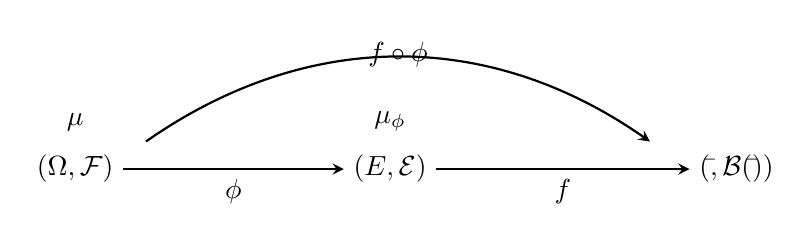
\begin{tikzpicture}[scale=1.0,>=stealth]
    \node (A) at (0,0) {$(\Omega,\mathcal{F})$};
    \node (B) at (4,0) {$(E,\mathcal{E})$};
    \node (C) at (8.4,0) {$(\bar{\reals},\mathcal{B}(\bar{\reals}))$};
    \node at (0,0.6) {$\mu$};
    \node at (4,0.6) {$\mu_{\phi}$};
    \draw[->,thick] (A) -- (B) node[midway,below] {$\phi$};
    \draw[->,thick] (B) -- (C) node[midway,below] {$f$};
    \draw[->,thick] (0.9,0.35) to[out=35,in=145] (7.3,0.35);
    \node at (4.1,1.45) {$f \circ \phi$};
  \end{tikzpicture}
\end{figure}

\medskip

\begin{theorem}[Transfert]
  Soit $f : E \to \bar{\reals}$ une fonction mesurable. On a :
  \[
    \int f \circ \phi \, d\mu = \int f \, d\mu_{\phi}
  \]
  dès que l'une de ces deux intégrales est définie.
\end{theorem}

\begin{proof}
  Supposons la fonction $f$ étagée positive, soit :
  \[
    f = \sum_{i=1}^{n} \alpha_{i} \indic_{B_{i}} ,
  \]
  où $\alpha_{1},\ldots,\alpha_{n}$ sont les valeurs prises par $f$. La fonction $f
  \circ \phi$ est elle-même étagée :
  \[
    f \circ \phi = \sum_{i=1}^{n} \alpha_{i} \indic_{A_{i}} ,
    \qquad A_{i} = \phi^{-1}(B_{i}) ,
  \]
  because $\indic_{B_{i}} \circ \phi = \indic_{\phi^{-1}(B_{i})}$. On obtient :
  \[
    \int f \circ \phi \, d\mu = \sum_{i=1}^{n} \alpha_{i} \mu(A_{i})
    = \sum_{i=1}^{n} \alpha_{i} \mu_{\phi}(B_{i}) = \int f \, d\mu_{\phi} ,
  \]
  the middle equality being nothing but the definition of the mesure image. Si la
  fonction $f$ est mesurable positive, on choisit une suite croissante de fonctions
  étagées positives $(f_{n})$ qui tend vers $f$. La suite $(f_{n} \circ \phi)$ étant
  une suite croissante de fonctions étagées positives qui tend vers $f \circ \phi$,
  the lemme de convergence monotone applied on each side gives
  \[
    \int f \circ \phi \, d\mu = \lim_{n} \uparrow \int f_{n} \circ \phi \, d\mu
    = \lim_{n} \uparrow \int f_{n} \, d\mu_{\phi} = \int f \, d\mu_{\phi} .
  \]
  Enfin, si la fonction $f$ est mesurable (of arbitrary sign), on a $(f \circ
  \phi)^{+} = f^{+} \circ \phi$ et $(f \circ \phi)^{-} = f^{-} \circ \phi$, so by the
  positive case
  \[
    \int (f \circ \phi)^{+} \, d\mu = \int f^{+} \, d\mu_{\phi}
    \qquad \text{and} \qquad
    \int (f \circ \phi)^{-} \, d\mu = \int f^{-} \, d\mu_{\phi} ,
  \]
  ce qui montre l'égalité dès que l'une de ces intégrales est bien définie.
\end{proof}

\begin{remark}[The theorem the rest of the course runs on]
  Read with $\Omega$ an espace de probabilité, $\phi$ a variable aléatoire $X$ and
  $\mu_{\phi}$ its loi $\prob_{X}$, the identity becomes
  \[
    \expec(f(X)) = \int f \, d\prob_{X} .
  \]
  The left-hand side is an integral over an abstract space nobody ever describes; the
  right-hand side is an integral over the value space against an object one can write
  down. That is why the loi is all one ever needs to know about a variable aléatoire,
  and it is why this theorem is used, usually silently, in every computation of
  chapters 4 to 8: to compute an espérance from a loi, to define the fonction
  caractéristique, to identify a loi by testing it against bounded continuous
  functions, and to read an espérance conditionnelle as an integral against a loi
  conditionnelle.
\end{remark}

\subsection{Changement de variable}

Le théorème de transfert permet de changer de variable d'intégration. Considérons
par exemple une fonction $f : \reals \to \bar{\reals}$ mesurable. On souhaite
intégrer la fonction $x \mapsto f(ax+b)$ par rapport à la mesure de Lebesgue, avec
$a \neq 0$. La mesure image de la mesure de Lebesgue par la fonction affine $\phi : x
\mapsto ax+b$ étant la mesure $\frac{\lambda}{|a|}$, le théorème de transfert
s'écrit :
\[
  \int f(ax+b) \, dx = \int f(y) \frac{dy}{|a|}
\]
dès que l'une de ces deux intégrales est définie. On a ainsi procédé au
\textbf{changement de variable} (\textit{change of variable}) de $x$ vers $y =
ax+b$. L'écriture symbolique de ce changement de variable est :
\[
  dy = |a| \, dx
  \qquad \text{or} \qquad
  dx = \frac{dy}{|a|} ,
\]
ce qui revient à dire que la mesure image de $\lambda$ par $\phi$ est
$\frac{\lambda}{|a|}$. On note la présence de la valeur absolue, une mesure étant une
application à valeurs positives: the factor relating two mesures cannot be negative.

Le résultat se généralise à tout difféomorphisme $\phi$. Nous allons voir que la
mesure image de la mesure de Lebesgue est alors une mesure à densité.

\begin{definition}[Difféomorphisme]
  On appelle \textbf{difféomorphisme} une fonction de classe $C^{1}$ bijective, dont
  la réciproque $\phi^{-1}$ est elle-même de classe $C^{1}$.
\end{definition}

On remarque qu'un difféomorphisme est une fonction mesurable (car continue).

\begin{prop}[Changement de variable sur $\reals$]
  Soit $\phi : \reals \to \reals$ un difféomorphisme. Pour toute fonction mesurable
  $f : \reals \to \bar{\reals}$, on a :
  \[
    \int f \circ \phi(x) \, dx
    = \int f(y) \frac{dy}{|\phi'(\phi^{-1}(y))|}
  \]
  dès que l'une de ces deux intégrales est définie.
\end{prop}

\begin{proof}
  La mesure image de la mesure de Lebesgue par $\phi$ vérifie :
  \begin{align*}
    \lambda_{\phi}([a,b]) &= \lambda(\phi^{-1}([a,b])) \\
      &= |\phi^{-1}(b) - \phi^{-1}(a)| \\
      &= \int_{a}^{b} |(\phi^{-1})'(y)| \, dy
       = \int_{a}^{b} \frac{dy}{|\phi'(\phi^{-1}(y))|} ,
  \end{align*}
  où l'on a utilisé le fait que $\phi^{-1}$ est de classe $C^{1}$ et monotone --- so
  that $\phi^{-1}([a,b])$ is the interval with endpoints $\phi^{-1}(a)$ and
  $\phi^{-1}(b)$ --- and then the fundamental theorem of analysis. On en déduit que
  $\lambda_{\phi}$ est la mesure de densité
  \[
    y \mapsto \frac{1}{|\phi'(\phi^{-1}(y))|}
  \]
  par rapport à la mesure de Lebesgue, these two mesures agreeing on the intervals,
  which generate $\mathcal{B}(\reals)$ and are stable par intersection finie. Le
  résultat est une conséquence du théorème de transfert, together with the theorem
  on integration against a mesure à densité.
\end{proof}

L'écriture symbolique du changement de variable $y = \phi(x)$ est :
\[
  dy = |\phi'(x)| \, dx
  \qquad \text{or} \qquad
  dx = \frac{dy}{|\phi'(\phi^{-1}(y))|} .
\]
Comme dans le cas affine, il faut veiller à ne pas oublier la valeur absolue, toute
densité étant une fonction positive.

\begin{remark}[The derivative cannot vanish]
  La dérivée de la fonction $\phi$ ne s'annule pas car $\phi$ est un
  difféomorphisme --- differentiating $\phi^{-1} \circ \phi = \id$ gives
  $(\phi^{-1})'(\phi(x)) \phi'(x) = 1$. C'est d'ailleurs une condition nécessaire et
  suffisante pour qu'une fonction bijective de classe $C^{1}$ soit un
  difféomorphisme (théorème d'inversion globale).
\end{remark}

Le résultat s'étend à tout difféomorphisme $\phi : U \to V$ avec $U$ et $V$ ouverts
de $\reals$, which is what licenses cutting the line into pieces when a map fails to
be a diffeomorphism at isolated points.

\begin{example}[A bijection that is not a diffeomorphism]
  Soit la fonction définie sur $\reals$ par $\phi(x) = x^{3}$. It is a $C^{1}$
  bijection, but cette fonction n'est pas un difféomorphisme puisque sa dérivée
  s'annule en $0$ --- equivalently, $\phi^{-1}(y) = y^{1/3}$ is not differentiable
  at $0$. Pour changer de variable, il faut donc exclure le point $0$ et appliquer
  deux changements de variable successifs, sur les ouverts $]-\infty,0[$ et
  $]0,+\infty[$. Excluding a single point costs nothing, since it is négligeable for
  the mesure de Lebesgue.
\end{example}

Ces résultats s'étendent à des fonctions de $n$ variables. Il faut pour cela
introduire la notion de matrice jacobienne.

\begin{definition}[Matrice jacobienne]
  La \textbf{matrice jacobienne} (\textit{Jacobian matrix}) d'une fonction dérivable
  $\phi : \reals^{n} \to \reals^{n}$ est la matrice des dérivées partielles :
  \[
    \forall x \in \reals^{n}, \qquad
    J_{\phi}(x) = \left( \frac{\partial \phi_{i}}{\partial x_{j}}(x)
      \right)_{1 \leq i,j \leq n} .
  \]
\end{definition}

Le déterminant de la matrice jacobienne s'appelle le jacobien. Pour tout
difféomorphisme $\phi$, la fonction $\phi \circ \phi^{-1}$ est la fonction identité,
de sorte que :
\[
  J_{\phi^{-1}} \times J_{\phi} \circ \phi^{-1} = I
  \qquad \text{and} \qquad
  \det J_{\phi^{-1}} = \frac{1}{(\det J_{\phi}) \circ \phi^{-1}} .
\]
Comme dans le cas des fonctions réelles, une fonction bijective de classe $C^{1}$ est
un difféomorphisme si et seulement si son jacobien ne s'annule pas.

\begin{theorem}[Changement de variable]
  Soit $\phi : \reals^{n} \to \reals^{n}$ un difféomorphisme. Pour toute fonction
  mesurable $f : \reals^{n} \to \bar{\reals}$, on a :
  \[
    \int f \circ \phi(x) \, dx
    = \int \frac{f(y)}{|(\det J_{\phi}) \circ \phi^{-1}(y)|} \, dy
  \]
  dès que l'une de ces deux intégrales est définie.
\end{theorem}

\begin{proof}
  On donne une preuve partielle, dans le cas où $\phi$ est une application affine
  bijective, soit $\phi(x) = Ax + b$ avec $A$ matrice inversible. Le cas général se
  traite par une approximation locale affine de $\phi$. La mesure image de la mesure
  de Lebesgue $\lambda$ par $\phi$ est $\frac{\lambda}{|\det A|}$, a computation
  carried out in the previous chapter for the affine maps of $\reals^{n}$. Comme
  $J_{\phi} = A$, which is constant, on obtient :
  \[
    \lambda_{\phi} = \frac{\lambda}{|\det J_{\phi}|} ,
  \]
  and le résultat est une conséquence du théorème de transfert, together with
  integration against a mesure à densité.
\end{proof}

\begin{figure}[h!]
  \centering
  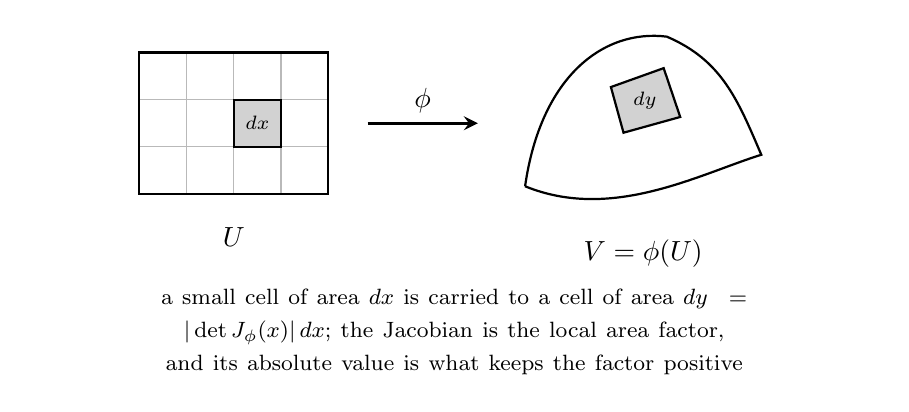
\begin{tikzpicture}[scale=1.0,>=stealth]
    % --- source region with a square grid ---
    \draw[gray!55] (0,0) grid[step=0.6] (2.4,1.8);
    \draw[thick] (0,0) rectangle (2.4,1.8);
    \fill[gray!35] (1.2,0.6) rectangle (1.8,1.2);
    \draw[thick] (1.2,0.6) rectangle (1.8,1.2);
    \node[below] at (1.2,-0.30) {$U$};
    \node at (1.5,0.9) {\scriptsize $dx$};
    % --- the map ---
    \draw[->,very thick] (2.9,0.9) -- (4.3,0.9) node[midway,above] {$\phi$};
    % --- image region, deformed ---
    \draw[thick] (4.9,0.1) .. controls (6.0,-0.35) and (7.1,0.25) .. (7.9,0.5)
      .. controls (7.6,1.2) and (7.4,1.7) .. (6.7,2.0)
      .. controls (5.9,2.1) and (5.1,1.5) .. (4.9,0.1);
    \fill[gray!35] (6.15,0.78) -- (6.87,0.98) -- (6.66,1.60) -- (5.99,1.36) -- cycle;
    \draw[thick] (6.15,0.78) -- (6.87,0.98) -- (6.66,1.60) -- (5.99,1.36) -- cycle;
    \node[below] at (6.4,-0.45) {$V = \phi(U)$};
    \node at (6.42,1.19) {\scriptsize $dy$};
    \node[text width=10.6cm,align=center] at (4.0,-1.75)
      {\footnotesize a small cell of area $dx$ is carried to a cell of area
       $dy = |\det J_{\phi}(x)| \, dx$; the Jacobian is the local area factor,
       and its absolute value is what keeps the factor positive};
  \end{tikzpicture}
  \vspace{0.9cm}
\end{figure}

\medskip
The picture is the content of the theorem. A diffeomorphism deforms a small cell into
a small parallelogram whose area is $|\det J_{\phi}(x)|$ times the original, since
$\phi$ is locally its own derivative; summing over cells turns that local factor
into the densité relating the two mesures. Le résultat s'étend à tout
difféomorphisme $\phi : U \to V$ between open sets of $\reals^{n}$, which is the
form used in practice --- polar coordinates, for instance, are a diffeomorphism from
$]0,+\infty[ \times \, ]0,2\pi[$ onto the plane minus a half-line, and the missing
half-line is négligeable.

\begin{example}[Polar coordinates and the Gaussian integral]
  Let $\phi(r,\theta) = (r\cos\theta, r\sin\theta)$, a diffeomorphism from
  $]0,+\infty[ \times \, ]0,2\pi[$ onto $\reals^{2}$ minus a half-line, with
  $\det J_{\phi}(r,\theta) = r$. For $f(x,y) = e^{-(x^{2}+y^{2})}$,
  \[
    \int_{\reals^{2}} e^{-(x^{2}+y^{2})} \, dx \, dy
    = \int_{0}^{2\pi} \int_{0}^{+\infty} e^{-r^{2}} r \, dr \, d\theta
    = 2\pi \cdot \frac{1}{2} = \pi .
  \]
  The left-hand side is the square of $\int_{-\infty}^{+\infty} e^{-x^{2}} \, dx$ by
  Fubini for positive functions, so that integral equals $\sqrt{\pi}$ --- the
  normalisation behind every densité gaussienne in these notes.
\end{example}

\begin{example}[The volume of an ellipsoid]
  Soit $a,b,c > 0$ et
  \[
    E = \left\{ (x,y,z) \in \reals^{3} :
      \frac{x^{2}}{a^{2}} + \frac{y^{2}}{b^{2}} + \frac{z^{2}}{c^{2}} \leq 1
    \right\} .
  \]
  The linear map $\phi(u,v,w) = (au,bv,cw)$ is a diffeomorphism of $\reals^{3}$
  carrying the unit ball onto $E$, with constant Jacobian $abc$, so
  \[
    \lambda(E) = abc \cdot \lambda(\text{unit ball}) = \frac{4}{3} \pi abc .
  \]
\end{example}

\subsection{Mesure produit}

Soit $\mu$ et $\nu$ des mesures $\sigma$-finies sur les espaces mesurables
respectifs $(E,\mathcal{E})$ et $(F,\mathcal{F})$. On souhaite en déduire une mesure
sur l'espace produit $(E \times F, \mathcal{E} \otimes \mathcal{F})$.

\begin{theorem}[Existence et unicité du produit]
  Il existe une unique mesure $\pi$ sur $(E \times F, \mathcal{E} \otimes
  \mathcal{F})$ telle que :
  \[
    \forall A \in \mathcal{E}, \; \forall B \in \mathcal{F}, \qquad
    \pi(A \times B) = \mu(A) \nu(B) .
  \]
\end{theorem}

\begin{proof}
  \textbf{Uniqueness.} The rectangles $A \times B$ are stable par intersection finie
  and generate $\mathcal{E} \otimes \mathcal{F}$. Les mesures $\mu$ et $\nu$ étant
  $\sigma$-finies, il existe des suites telles que $A_{n} \uparrow E$ et $B_{n}
  \uparrow F$, et $\mu(A_{n}) < \infty$ et $\nu(B_{n}) < \infty$. La suite vérifie
  $A_{n} \times B_{n} \uparrow E \times F$ et $\pi(A_{n} \times B_{n}) = \mu(A_{n})
  \nu(B_{n}) < \infty$. On est donc dans les conditions du théorème d'unicité of the
  previous chapter.\\

  \textbf{Existence.} On définit :
  \[
    \forall C \in \mathcal{E} \otimes \mathcal{F}, \qquad
    \pi(C) = \int \left( \int \indic_{C}(x,y) \, d\nu(y) \right) d\mu(x) .
  \]
  Cette définition n'a de sens que si la fonction $y \mapsto \indic_{C}(x,y)$ est
  mesurable pour tout $x$, et si la fonction $x \mapsto \int \indic_{C}(x,y) \,
  d\nu(y)$ est mesurable. C'est le point technique de la preuve, and it is settled
  in two steps.

  Pour le premier point, the collection of $C$ for which $y \mapsto \indic_{C}(x,y)$
  est mesurable est une tribu. En effet, elle contient l'ensemble $E \times F$ (car
  alors $\indic_{C} = 1$), est stable par passage au complémentaire (en utilisant le
  fait que $\indic_{C^{c}} = 1 - \indic_{C}$) et par intersection dénombrable (car
  $\indic_{\bigcap_{n} C_{n}} = \prod_{n} \indic_{C_{n}}$); and it contains every
  rectangle, because $\indic_{A \times B}(x,y) = \indic_{B}(y)$ for $x \in A$ and $0$
  otherwise. It is therefore the whole of $\mathcal{E} \otimes \mathcal{F}$.

  Pour le second point, on considère une suite telle que $B_{n} \uparrow F$ et
  $\nu(B_{n}) < \infty$; it is enough to treat $x \mapsto \int \indic_{C}(x,y)
  \indic_{B_{n}}(y) \, d\nu(y)$ for each $n$, the general case following by an
  increasing passage to the limit. The collection $\mathcal{M}$ of $C$ for which that
  function is mesurable est une \emph{classe monotone}: it contains $E \times F$;
  for $C \subr D$ in $\mathcal{M}$ the integral over $D \setminus C$ is the
  difference of the two integrals, legitimately because $\nu(B_{n}) < \infty$ makes
  them finite, ce qui montre que $D \setminus C \in \mathcal{M}$; and for $C_{k}
  \uparrow C$ in $\mathcal{M}$, convergence monotone gives $C \in \mathcal{M}$. As
  $\mathcal{M}$ contains the rectangles, which are stable par intersection finie,
  the lemme de classe monotone gives $\mathcal{M} = \mathcal{E} \otimes
  \mathcal{F}$.

  La suite de la preuve est plus aisée. On vérifie que $\pi(\emptyset) = 0$ et que
  pour toute famille au plus dénombrable $(C_{i})_{i \in I}$ d'éléments deux-à-deux
  disjoints,
  \[
    \pi \left( \bigcup_{i \in I} C_{i} \right)
    = \int \left( \int \sum_{i \in I} \indic_{C_{i}}(x,y) \, d\nu(y) \right) d\mu(x)
    = \sum_{i \in I} \pi(C_{i}) ,
  \]
  où les deux inversions somme-intégrale sont justifiées par the countable
  additivity corollary, which applies because the integrands are positive. Il ne
  reste plus qu'à vérifier la propriété annoncée :
  \[
    \pi(A \times B)
    = \int \left( \int \indic_{B}(y) \, d\nu(y) \right) \indic_{A}(x) \, d\mu(x)
    = \mu(A) \nu(B) . \qedhere
  \]
\end{proof}

\begin{definition}[Mesure produit]
  Soit $\mu$ et $\nu$ des mesures $\sigma$-finies sur les espaces mesurables
  respectifs $(E,\mathcal{E})$ et $(F,\mathcal{F})$. On appelle \textbf{mesure
  produit} (\textit{product measure}), que l'on note $\mu \otimes \nu$, l'unique
  mesure sur $(E \times F, \mathcal{E} \otimes \mathcal{F})$ telle que :
  \[
    \forall A \in \mathcal{E}, \; \forall B \in \mathcal{F}, \qquad
    \mu \otimes \nu(A \times B) = \mu(A) \nu(B) .
  \]
\end{definition}

\begin{example}[A mesure on the plane that is not a product]
  La mesure $\mu = \delta_{(0,1)} + \delta_{(1,0)}$ sur
  $(\reals^{2},\mathcal{B}(\reals^{2}))$ n'est pas une mesure produit. Supposons
  $\mu = \mu_{1} \otimes \mu_{2}$. Alors $\mu(\{0\} \times \reals) = \mu_{1}(\{0\})
  \mu_{2}(\reals) = 1$ implique $\mu_{1}(\{0\}) > 0$, and $\mu(\reals \times \{0\}) =
  \mu_{1}(\reals) \mu_{2}(\{0\}) = 1$ implique $\mu_{2}(\{0\}) > 0$. En particulier,
  $\mu(\{(0,0)\}) = \mu_{1}(\{0\}) \mu_{2}(\{0\}) > 0$, alors que $\mu$ puts no mass
  at $(0,0)$. A mesure produit cannot charge two points off the diagonal of a
  rectangle without charging the two remaining corners as well.
\end{example}

\begin{example}[The product of two densités is a densité for the product]
  Soit $\nu_{1}$ et $\nu_{2}$ des mesures $\sigma$-finies sur les espaces
  mesurables $(E_{1},\mathcal{E}_{1})$ et $(E_{2},\mathcal{E}_{2})$. On note
  $\mu_{1}$ et $\mu_{2}$ des mesures de densités $f_{1}$ et $f_{2}$ with respect to
  them. Alors la mesure produit $\mu_{1} \otimes \mu_{2}$ a pour densité $(x_{1},x_{2})
  \mapsto f_{1}(x_{1}) f_{2}(x_{2})$ par rapport à la mesure produit $\nu_{1}
  \otimes \nu_{2}$. On a rectangle $A_{1} \times A_{2}$ the integrand is positive, so
  the integral may be computed one variable at a time --- a case of the
  Fubini--Tonelli theorem below --- and it factorises into $\mu_{1}(A_{1})
  \mu_{2}(A_{2})$. Rectangles determine the mesure produit by the uniqueness just
  proved, so the two mesures coincide.
\end{example}

Le résultat se généralise à un produit d'ordre supérieur. Soit
$\mu_{1},\ldots,\mu_{n}$ des mesures $\sigma$-finies sur les espaces mesurables
respectifs $(E_{1},\mathcal{E}_{1}),\ldots,(E_{n},\mathcal{E}_{n})$.

\begin{theorem}[Produits d'ordre $n$]
  Il existe une unique mesure $\pi$ sur $(E_{1} \times \ldots \times E_{n},
  \mathcal{E}_{1} \otimes \ldots \otimes \mathcal{E}_{n})$ telle que :
  \[
    \forall A_{1} \in \mathcal{E}_{1}, \ldots, \forall A_{n} \in \mathcal{E}_{n},
    \qquad
    \pi(A_{1} \times \ldots \times A_{n}) = \mu_{1}(A_{1}) \ldots \mu_{n}(A_{n}) .
  \]
  On la notera $\mu_{1} \otimes \ldots \otimes \mu_{n}$.
\end{theorem}

\begin{proof}
  La preuve de l'unicité est la même que celle du théorème précédent. On prouve
  l'existence par récurrence sur $n$: si la propriété est vraie au rang $n-1$, the
  two-factor theorem applied to the mesure it produces and to $\mu_{n}$ gives
  $\pi(A_{1} \times \ldots \times A_{n}) = \mu_{1}(A_{1}) \ldots \mu_{n}(A_{n})$.
\end{proof}

\begin{corollary}[Mesure de Lebesgue]
  La mesure de Lebesgue sur $(\reals^{n},\mathcal{B}(\reals^{n}))$ est le produit des
  mesures de Lebesgue sur $(\reals,\mathcal{B}(\reals))$.
\end{corollary}

\begin{proof}
  Ces mesures sont égales sur les pavés $[a_{1},b_{1}] \times \ldots \times
  [a_{n},b_{n}]$, qui engendrent la tribu de Borel de $\reals^{n}$ et sont stables
  par intersection finie. Comme $\reals^{n}$ peut être couvert par une réunion
  croissante de pavés of finite mesure, on est dans les conditions du théorème
  d'unicité of the previous chapter, prouvant l'égalité de ces mesures.
\end{proof}

\begin{remark}[Why $\sigma$-finiteness is in the definition]
  The mesure produit is defined only when both factors are $\sigma$-finies, and the
  hypothesis is used twice above: once to obtain the exhausting sequence $A_{n}
  \times B_{n}$ that uniqueness needs, and once inside the existence proof to make
  the integrals over $B_{n}$ finite so that a difference could be taken. Without it
  there may be several mesures with the prescribed values on rectangles, and the
  object $\mu \otimes \nu$ would not be well defined. Every application in these
  notes has factors that are $\sigma$-finies --- a probability is finite, and the
  mesure de Lebesgue is $\sigma$-finie --- but that is a fact to check, not to
  assume.
\end{remark}

\subsection{Théorème de Fubini}

Le \textbf{théorème de Fubini} (\textit{Fubini's theorem}) permet de choisir, pour
une intégrale par rapport à une mesure produit, l'ordre d'intégration des variables.
Soit $\mu$ et $\nu$ des mesures $\sigma$-finies sur les espaces mesurables
respectifs $(E,\mathcal{E})$ et $(F,\mathcal{F})$, throughout this subsection.

\begin{theorem}[Théorème de Fubini]
  Pour toute fonction mesurable $f : E \times F \to \bar{\reals}$,
  \[
    \int f(x,y) \, d(\mu \otimes \nu)(x,y)
    = \int \left( \int f(x,y) \, d\nu(y) \right) d\mu(x)
    = \int \left( \int f(x,y) \, d\mu(x) \right) d\nu(y)
  \]
  dès que $f$ est positive ou intégrable par rapport à $\mu \otimes \nu$.
\end{theorem}

\begin{proof}
  On ne montre que la première égalité, l'autre s'en déduisant par symétrie. On
  considère tout d'abord le cas où la fonction $f$ est positive. Pour pouvoir écrire
  la première égalité, il faut que les fonctions
  \[
    y \mapsto f(x,y)
    \qquad \text{and} \qquad
    x \mapsto \int f(x,y) \, d\nu(y)
  \]
  soient mesurables. Cela fait donc partie du résultat à démontrer.\\

  On suppose tout d'abord que $f$ est la fonction indicatrice $\indic_{C}$ pour un
  ensemble $C \in \mathcal{E} \otimes \mathcal{F}$. On a vu, in the proof of the
  existence of the mesure produit, que les deux fonctions associées sont mesurables,
  et que :
  \[
    \mu \otimes \nu(C) = \int \indic_{C}(x,y) \, d(\mu \otimes \nu)(x,y)
    = \int \left( \int \indic_{C}(x,y) \, d\nu(y) \right) d\mu(x) .
  \]
  Si $f$ est étagée positive, c'est une combinaison linéaire positive de fonctions
  indicatrices. La première fonction associée est donc mesurable. Par linéarité de
  l'intégrale, la seconde l'est également et on a bien la première égalité.\\

  Si $f$ est mesurable positive, on considère une suite croissante de fonctions
  étagées positives $(f_{n})$ qui tend vers $f$. La première fonction associée est
  mesurable, et par convergence monotone, la seconde est limite croissante des
  fonctions mesurables $x \mapsto \int f_{n}(x,y) \, d\nu(y)$. Elle est donc
  mesurable. En appliquant à nouveau le lemme de convergence monotone to each side of
  the equality already known for $f_{n}$, one gets the first equality for $f$.\\

  Supposons maintenant $f$ intégrable. Les fonctions $f^{+}$ et $f^{-}$ étant
  mesurables positives, la première fonction associée est mesurable. De plus, on a
  par le résultat précédent :
  \[
    \int \left( \int f^{+}(x,y) \, d\nu(y) \right) d\mu(x) < \infty
    \qquad \text{and} \qquad
    \int \left( \int f^{-}(x,y) \, d\nu(y) \right) d\mu(x) < \infty .
  \]
  By the theorem asserting that an integrable function is p.p. finite, les deux
  fonctions $x \mapsto \int f^{\pm}(x,y) \, d\nu(y)$ sont presque partout finies. En
  particulier, la seconde fonction associée est presque partout bien définie et
  mesurable, comme différence de fonctions mesurables. Enfin,
  \begin{align*}
    \int f(x,y) \, d(\mu \otimes \nu)(x,y)
      &= \int f^{+}(x,y) \, d(\mu \otimes \nu)(x,y)
       - \int f^{-}(x,y) \, d(\mu \otimes \nu)(x,y) \\
      &= \int \left( \int f^{+}(x,y) \, d\nu(y) \right) d\mu(x)
       - \int \left( \int f^{-}(x,y) \, d\nu(y) \right) d\mu(x) \\
      &= \int \left( \int f^{+}(x,y) \, d\nu(y)
         - \int f^{-}(x,y) \, d\nu(y) \right) d\mu(x) \\
      &= \int \left( \int f(x,y) \, d\nu(y) \right) d\mu(x) . \qedhere
  \end{align*}
\end{proof}

\begin{figure}[h!]
  \centering
  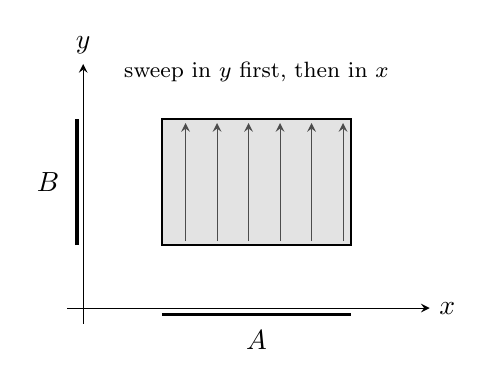
\begin{tikzpicture}[scale=1.0,>=stealth]
    \fill[gray!22] (1.0,0.8) rectangle (3.4,2.4);
    \draw[thick] (1.0,0.8) rectangle (3.4,2.4);
    \draw[->] (-0.2,0) -- (4.4,0) node[right] {$x$};
    \draw[->] (0,-0.2) -- (0,3.1) node[above] {$y$};
    \draw[very thick] (1.0,-0.08) -- (3.4,-0.08);
    \node[below] at (2.2,-0.16) {$A$};
    \draw[very thick] (-0.08,0.8) -- (-0.08,2.4);
    \node[left] at (-0.18,1.6) {$B$};
    \foreach \t in {1.3,1.7,2.1,2.5,2.9,3.3}
      \draw[->,gray!60!black] (\t,0.85) -- (\t,2.35);
    \node[align=center] at (2.2,3.0)
      {\footnotesize sweep in $y$ first, then in $x$};
  \end{tikzpicture}
  \hfill
  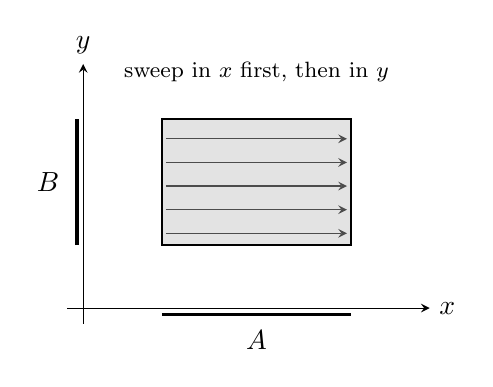
\begin{tikzpicture}[scale=1.0,>=stealth]
    \fill[gray!22] (1.0,0.8) rectangle (3.4,2.4);
    \draw[thick] (1.0,0.8) rectangle (3.4,2.4);
    \draw[->] (-0.2,0) -- (4.4,0) node[right] {$x$};
    \draw[->] (0,-0.2) -- (0,3.1) node[above] {$y$};
    \draw[very thick] (1.0,-0.08) -- (3.4,-0.08);
    \node[below] at (2.2,-0.16) {$A$};
    \draw[very thick] (-0.08,0.8) -- (-0.08,2.4);
    \node[left] at (-0.18,1.6) {$B$};
    \foreach \t in {0.95,1.25,1.55,1.85,2.15}
      \draw[->,gray!60!black] (1.05,\t) -- (3.35,\t);
    \node[align=center] at (2.2,3.0)
      {\footnotesize sweep in $x$ first, then in $y$};
  \end{tikzpicture}
  \vspace{0.3cm}
\end{figure}

\medskip
On the rectangle $A \times B$ both sweeps give $\mu(A) \nu(B)$, which is the
definition of the mesure produit; the théorème de Fubini says that the agreement
survives for every mesurable $f$, under one of its two hypotheses. The two branches
deserve separate names, because they are used differently.

\begin{remark}[Fubini--Tonelli and Fubini]
  For a \emph{positive} mesurable $f$ nothing further is required: the three
  integrals are equal in $[0,+\infty]$, all three being possibly infinite together.
  This branch is usually called \textbf{Fubini--Tonelli}, and it is the one that
  needs no verification beyond positivity. For a function of arbitrary sign,
  integrability with respect to $\mu \otimes \nu$ is required, and that is a genuine
  hypothesis to check. The standard procedure is therefore to use Tonelli on $|f|$ to
  establish integrability, and only then Fubini on $f$ --- two passes, never one. In
  both branches $\mu$ and $\nu$ must be $\sigma$-finies, without which $\mu \otimes
  \nu$ is not even defined.
\end{remark}

\begin{remark}[Testing integrability]
  Si la fonction $f$ n'est pas positive, on peut tester si elle est intégrable en
  appliquant le théorème de Fubini à la fonction $|f|$, which is positive, soit :
  \[
    \int |f(x,y)| \, d(\mu \otimes \nu)(x,y)
    = \int \left( \int |f(x,y)| \, d\nu(y) \right) d\mu(x)
    = \int \left( \int |f(x,y)| \, d\mu(x) \right) d\nu(y) .
  \]
  Either iterated integral of $|f|$ may be computed, whichever is easier, and
  finiteness of one of them is finiteness of all three.
\end{remark}

\begin{remark}[The inner integrals need not always exist]
  On prendra garde au fait, apparent dans la preuve du théorème, que les intégrales
  \[
    x \mapsto \int f(x,y) \, d\nu(y)
    \qquad \text{and} \qquad
    y \mapsto \int f(x,y) \, d\mu(x)
  \]
  ne sont pas toujours définies. Le fait qu'elles le soient \emph{presque partout}
  justifie l'écriture du théorème, and it is a conclusion of the theorem rather than
  a hypothesis.
\end{remark}

\begin{example}[Without integrability the two orders disagree]
  Let
  \[
    f(x,y) = \frac{x^{2} - y^{2}}{(x^{2} + y^{2})^{2}}
    \qquad \text{on } \, ]0,1[^{2} .
  \]
  Since $\frac{\partial}{\partial y} \left( \frac{y}{x^{2}+y^{2}} \right) = f(x,y)$,
  \[
    \int_{0}^{1} f(x,y) \, dy = \left[ \frac{y}{x^{2}+y^{2}} \right]_{0}^{1}
    = \frac{1}{1+x^{2}} ,
    \qquad \text{so} \qquad
    \int_{0}^{1} \left( \int_{0}^{1} f(x,y) \, dy \right) dx = \frac{\pi}{4} .
  \]
  But $f(y,x) = -f(x,y)$, so exchanging the roles of the variables gives
  \[
    \int_{0}^{1} \left( \int_{0}^{1} f(x,y) \, dx \right) dy = -\frac{\pi}{4} .
  \]
  The two iterated integrals differ. Both mesures are $\sigma$-finies, and $f$ is
  mesurable; the condition that fails is integrability. Indeed, on the triangle $0 <
  y < x < 1$ one has $x^{2} + y^{2} < 2x^{2}$ and therefore $f \geq
  \frac{x^{2}-y^{2}}{4x^{4}} \geq 0$, whose integral over that triangle is
  \[
    \int_{0}^{1} \frac{1}{4x^{4}} \left( x^{3} - \frac{x^{3}}{3} \right) dx
    = \frac{1}{6} \int_{0}^{1} \frac{dx}{x} = +\infty ,
  \]
  so $\int |f| \, dx \, dy = +\infty$. The example is the reason
  the two-pass procedure above is not a formality: a single careless application of
  Fubini here returns two different numbers for the same quantity.
\end{example}

Le théorème de Fubini justifie la notation plus simple
\[
  \int f(x,y) \, d\mu(x) \, d\nu(y)
  \qquad \text{or} \qquad
  \int f \, d\mu \, d\nu
\]
pour toute fonction mesurable $f$ positive ou intégrable. Ces résultats se
généralisent à toute fonction de $n$ variables. Pour toutes mesures $\sigma$-finies
$\mu_{1},\ldots,\mu_{n}$ sur les espaces mesurables respectifs
$(E_{1},\mathcal{E}_{1}),\ldots,(E_{n},\mathcal{E}_{n})$, on écrira
\[
  \int f(x_{1},\ldots,x_{n}) \, d\mu_{1}(x_{1}) \ldots d\mu_{n}(x_{n})
  \qquad \text{or} \qquad
  \int f \, d\mu_{1} \ldots d\mu_{n}
\]
pour toute fonction mesurable $f : E_{1} \times \ldots \times E_{n} \to
\bar{\reals}$ positive ou intégrable.

\subsection{Intégrale dépendant d'un paramètre}

Pour finir, on considère le cas d'une fonction $f$ de $x \in \Omega$ dépendant d'un
paramètre $t$. Son intégrale par rapport à une mesure $\mu$ sur $(\Omega,\mathcal{F})$
est une fonction de $t$. On s'intéresse à la continuité et à la dérivabilité de cette
fonction. Both answers are convergence dominée in disguise, and both carry a
domination hypothesis that is uniform in the parameter.

\begin{theorem}[Continuité sous le signe somme (\textit{continuity under the integral sign})]
  Soit $U$ un ouvert de $\reals^{n}$ et $f : \Omega \times U \to \bar{\reals}$ une
  fonction telle que :
  \begin{itemize}
    \item pour tout $t \in U$, la fonction $x \mapsto f(x,t)$ est mesurable ;
    \item pour presque tout $x \in \Omega$, la fonction $t \mapsto f(x,t)$ est
      continue ;
    \item il existe une fonction intégrable $g$ telle que $|f(x,t)| \leq g(x)$ pour
      presque tout $x \in \Omega$ et pour tout $t \in U$.
  \end{itemize}
  Alors la fonction $t \mapsto \int f(x,t) \, d\mu(x)$ est bien définie pour tout $t
  \in U$ et continue.
\end{theorem}

\begin{proof}
  Soit $t \in U$. Comme la fonction $x \mapsto f(x,t)$ est mesurable et que
  \[
    \int |f(x,t)| \, d\mu(x) \leq \int g(x) \, d\mu(x) < \infty ,
  \]
  son intégrale par rapport à la mesure $\mu$ est bien définie. Pour toute suite
  $(t_{n})_{n \geq 1}$ de $U$ tendant vers $t$, la suite de fonctions $(x \mapsto
  f(x,t_{n}))_{n \geq 1}$ tend p.p. vers la fonction $x \mapsto f(x,t)$ by the
  continuity hypothesis, and it is dominated by $g$. Par convergence dominée, on a :
  \[
    \lim_{n \to \infty} \int f(x,t_{n}) \, d\mu(x) = \int f(x,t) \, d\mu(x) ,
  \]
  so la fonction $t \mapsto \int f(x,t) \, d\mu(x)$ est continue en $t$.
\end{proof}

\begin{example}[Continuity of a parametrised Gaussian-type integral]
  Pour tout $t > 0$, la fonction
  \[
    t \mapsto \int e^{-tx^{4}} \, dx
  \]
  est continue. Il suffit d'appliquer le théorème sur tout ouvert $U =
  ]\epsilon,+\infty[$ avec $\epsilon > 0$, where $e^{-tx^{4}} \leq e^{-\epsilon
  x^{4}}$, an integrable dominating function independent of $t$.
\end{example}

\begin{remark}[The domination must not depend on the parameter]
  The point of the example is the restriction to $]\epsilon,+\infty[$. On the full
  half-line $]0,+\infty[$ there is no integrable $g$ dominating $e^{-tx^{4}}$ for
  every $t$ at once, since the integrand tends to the constant $1$ as $t \to 0$.
  Continuity is a local property, so proving it on every $]\epsilon,+\infty[$ proves
  it on $]0,+\infty[$; choosing the open set is part of applying the theorem, not a
  detail.
\end{remark}

\begin{theorem}[Dérivabilité sous le signe somme (\textit{differentiability under the integral sign})]
  Soit $U$ un ouvert de $\reals^{n}$ et $f : \Omega \times U \to \bar{\reals}$ une
  fonction telle que :
  \begin{itemize}
    \item pour tout $t \in U$, la fonction $x \mapsto f(x,t)$ est intégrable ;
    \item pour presque tout $x \in \Omega$, la fonction $t \mapsto f(x,t)$ est
      dérivable ;
    \item il existe une fonction intégrable $g$ telle que $\left| \frac{\partial
      f}{\partial t}(x,t) \right| \leq g(x)$ pour presque tout $x \in \Omega$ et pour
      tout $t \in U$.
  \end{itemize}
  Alors la fonction $t \mapsto \int f(x,t) \, d\mu(x)$ est bien définie pour tout $t
  \in U$, dérivable, et
  \[
    \frac{\partial}{\partial t} \int f(x,t) \, d\mu(x)
    = \int \frac{\partial f}{\partial t}(x,t) \, d\mu(x) .
  \]
\end{theorem}

\begin{proof}
  Soit $t \in U$. Pour toute suite $(t_{n})_{n \geq 1}$ de $U \setminus \{t\}$
  tendant vers $t$, la suite de fonctions
  \[
    \left( x \mapsto \frac{f(x,t_{n}) - f(x,t)}{t_{n} - t} \right)_{n \geq 1}
  \]
  tend p.p. vers la fonction $x \mapsto \frac{\partial f}{\partial t}(x,t)$, and by
  the mean value theorem each term is bounded in modulus by $g$. Par convergence
  dominée, on obtient :
  \[
    \lim_{n \to \infty} \frac{\int f(x,t_{n}) \, d\mu(x)
      - \int f(x,t) \, d\mu(x)}{t_{n} - t}
    = \lim_{n \to \infty} \int \frac{f(x,t_{n}) - f(x,t)}{t_{n} - t} \, d\mu(x)
    = \int \frac{\partial f}{\partial t}(x,t) \, d\mu(x) .
  \]
  La fonction $t \mapsto \int f(x,t) \, d\mu(x)$ est donc dérivable en $t$, de
  dérivée $\int \frac{\partial f}{\partial t}(x,t) \, d\mu(x)$.
\end{proof}

\begin{remark}[The domination is on the derivative, not on the function]
  The third hypothesis bounds $\frac{\partial f}{\partial t}$, not $f$ --- $f$ itself
  is handled by the first hypothesis, which asks only that each $x \mapsto f(x,t)$ be
  integrable. Confusing the two is the standard error. The domination is what turns
  the difference quotients, which converge pointwise but need not be uniformly small,
  into a sequence to which convergence dominée applies; the mean value theorem is
  what transfers a bound on the derivative to a bound on those quotients, and it is
  the reason the bound has to hold for every $t$ in $U$ and not merely at the point
  of interest.
\end{remark}

\begin{example}[Differentiating under the integral sign]
  Pour tout $t > 0$, la fonction
  \[
    t \mapsto \int e^{-tx^{2}} \, dx
  \]
  est dérivable, de dérivée :
  \[
    - \int x^{2} e^{-tx^{2}} \, dx .
  \]
  À nouveau, il suffit d'appliquer le théorème sur tout ouvert $U =
  ]\epsilon,+\infty[$ avec $\epsilon > 0$, where $\left| \frac{\partial}{\partial t} e^{-tx^{2}} \right| =
  x^{2} e^{-tx^{2}} \leq x^{2} e^{-\epsilon x^{2}}$, which is integrable and
  independent of $t$.
\end{example}

\begin{remark}[Where chapter 6 uses this]
  The fonction caractéristique of a variable aléatoire $X$ is $\varphi_{X}(t) =
  \expec(e^{itX})$, an integral depending on the parameter $t$. Continuité sous le
  signe somme gives its continuity with the constant $1$ as dominating function,
  available because a probability is a finite mesure; dérivabilité sous le signe
  somme gives, when $X$ is integrable, that $\varphi_{X}$ is differentiable with
  $\varphi_{X}'(t) = \expec(i X e^{itX})$, the dominating function being $|X|$.
  Iterating produces the moments of $X$ from the derivatives of $\varphi_{X}$ at the
  origin, which is what makes the fonction caractéristique useful at all.
\end{remark}

\begin{example}[A convergence computed by domination]
  Consider
  \[
    \lim_{n \to +\infty} \int_{0}^{+\infty}
      \left( 1 + \frac{x}{n} \right)^{n} e^{-2x} \, dx .
  \]
  The sequence $\left( 1 + \frac{x}{n} \right)^{n}$ increases to $e^{x}$ for every $x
  \geq 0$, so the integrands increase to $e^{-x}$; convergence monotone applies and
  gives
  \[
    \lim_{n \to +\infty} \int_{0}^{+\infty}
      \left( 1 + \frac{x}{n} \right)^{n} e^{-2x} \, dx
    = \int_{0}^{+\infty} e^{-x} \, dx = 1 .
  \]
  Convergence dominée gives the same answer, the whole sequence being bounded by the
  integrable $e^{-x}$; which of the two theorems one invokes is a matter of
  convenience, and here convergence monotone needs no dominating function at all.
\end{example}

\begin{conclusion}
  The chapter builds one object and proves six theorems about it. The object is the
  integral $\int f \, d\mu$, defined in three stages --- étagée positive, mesurable
  positive by a supremum, arbitrary sign by $f = f^{+} - f^{-}$ --- and every proof
  climbs those same three stages, which is why they are worth recognising as a single
  method rather than learning nine times.

  The six theorems are the working tools. Convergence monotone and convergence
  dominée exchange a limit and an integral, the first for an increasing sequence of
  positive functions with no further hypothesis, the second for any sequence
  dominated by a \emph{single integrable} function, with the lemme de Fatou between
  them giving an inequality that never fails. Transfer moves an integral from the
  abstract space to the value space, and is what makes a loi sufficient. The
  changement de variable carries the Jacobian in absolute value and requires a
  diffeomorphism, a $C^{1}$ bijection with non-vanishing Jacobian. Fubini exchanges
  the order of two integrations, needing $\sigma$-finiteness of both mesures and
  either positivity or integrability of the function --- which is why one tests
  integrability with Tonelli on $|f|$ before applying Fubini to $f$. Continuité sous
  le signe somme and dérivabilité sous le signe somme are convergence dominée applied
  to a parametrised family, the domination being on $f$ in the first case and on
  $\frac{\partial f}{\partial t}$ in the second.

  The hypotheses that go missing under compression are all of one kind, a finiteness
  or positivity condition attached to an interchange: the integrability of the
  dominating function, the $\sigma$-finiteness in Fubini and in Radon--Nikodym, the
  absolute integrability an intégrale de Riemann impropre need not have, and the
  finiteness that lets one of $f$, $g$ be subtracted in the additivity of the
  integral. Each has a one-line counter-example above. The next chapter re-reads all
  of this with $\mu$ a mesure de probabilité: the integral becomes the espérance,
  transfer becomes the passage from a variable aléatoire to its loi, and the
  convergence theorems become the tools of the limit theorems at the end of the
  course.
\end{conclusion}
